%%\documentclass[twocolumn]{aastex701}
%DIF LATEXDIFF DIFFERENCE FILE
%DIF DEL ../fields-goodman-2025-first-resubmission/main.tex   Mon Oct 26 04:09:15 2026
%DIF ADD main.tex                                             Mon Oct 26 08:55:30 2026
\documentclass[linenumbers]{aastex701}
%%\usepackage{graphicx} % Required for inserting images
\usepackage{url}
\usepackage{longtable}
\usepackage{csquotes} %DIF > 
\usepackage{overpic} %DIF > 
\usepackage{siunitx} %DIF > 
%DIF PREAMBLE EXTENSION ADDED BY LATEXDIFF
%DIF BOLD PREAMBLE %DIF PREAMBLE
\DeclareOldFontCommand{\bf}{\normalfont\bfseries}{\mathbf} %DIF PREAMBLE
\providecommand{\DIFadd}[1]{{\bf #1}} %DIF PREAMBLE
\providecommand{\DIFdel}[1]{} %DIF PREAMBLE
%DIF SAFE PREAMBLE %DIF PREAMBLE
\providecommand{\DIFaddbegin}{} %DIF PREAMBLE
\providecommand{\DIFaddend}{} %DIF PREAMBLE
\providecommand{\DIFdelbegin}{} %DIF PREAMBLE
\providecommand{\DIFdelend}{} %DIF PREAMBLE
\providecommand{\DIFmodbegin}{} %DIF PREAMBLE
\providecommand{\DIFmodend}{} %DIF PREAMBLE
%DIF FLOATSAFE PREAMBLE %DIF PREAMBLE
\providecommand{\DIFaddFL}[1]{\DIFadd{#1}} %DIF PREAMBLE
\providecommand{\DIFdelFL}[1]{\DIFdel{#1}} %DIF PREAMBLE
\providecommand{\DIFaddbeginFL}{} %DIF PREAMBLE
\providecommand{\DIFaddendFL}{} %DIF PREAMBLE
\providecommand{\DIFdelbeginFL}{} %DIF PREAMBLE
\providecommand{\DIFdelendFL}{} %DIF PREAMBLE
%DIF LISTINGS PREAMBLE %DIF PREAMBLE
\RequirePackage{listings} %DIF PREAMBLE
\lstdefinelanguage{DIFcode}{ %DIF PREAMBLE
%DIF DIFCODE_BOLD %DIF PREAMBLE
  % unfortunately \bfseries cannot be combined with ttfamily without extra packages %DIF PREAMBLE
  % also morecomment=[il] is broken as of v1.5b of listings at least %DIF PREAMBLE
  % workaround: plot in white with tiny font %DIF PREAMBLE
  % morecomment=[il]{\%DIF\ <\ }, %DIF PREAMBLE
  moredelim=[il][\color{white}\tiny]{\%DIF\ <\ }, %DIF PREAMBLE
  moredelim=[il][\sffamily\bfseries]{\%DIF\ >\ } %DIF PREAMBLE
} %DIF PREAMBLE
\lstdefinestyle{DIFverbatimstyle}{ %DIF PREAMBLE
	language=DIFcode, %DIF PREAMBLE
	basicstyle=\ttfamily, %DIF PREAMBLE
	columns=fullflexible, %DIF PREAMBLE
	keepspaces=true %DIF PREAMBLE
} %DIF PREAMBLE
\lstnewenvironment{DIFverbatim}{\lstset{style=DIFverbatimstyle}}{} %DIF PREAMBLE
\lstnewenvironment{DIFverbatim*}{\lstset{style=DIFverbatimstyle,showspaces=true}}{} %DIF PREAMBLE
\lstset{extendedchars=\true,inputencoding=utf8}

%DIF END PREAMBLE EXTENSION ADDED BY LATEXDIFF

\begin{document}

\title{A 2821 Star Optical SETI Survey using ESO HARPS archival data}
\author[0009-0008-7048-916X]{Benjamin Fields} %https://orcid.org/0009-0008-7048-916X
\affiliation{Southeastern Universities Research Association, 1201 New York Ave., NW, Suite 430, Washington, DC 20005}
\affiliation{Planetary Environments Labratory, Division 699, NASA Goddard Space Flight Center (GSFC), 8800 Greenbelt Road Greenbelt, MD 20771, USA}
\affiliation{Sellers Exoplanet Environments Collaboration (SEEC)}
\email{benjamin.l.fields@nasa.gov}
\email{bnfields72@gmail.com}

\author[0000-0002-6755-2710]{Jason C. Goodman}
\affiliation{Wheaton College, Norton MA USA}
\email{goodman_jason@wheatoncollege.edu}

\correspondingauthor{Benjamin L. Fields}
\email{bnfields72@gmail.com}
\date{July 2026}

\begin{abstract}
We examined archived observations of 2,821 stars taken by the high-resolution ESO HARPS spectrograph to search for potential narrow-band laser emissions from extraterrestrial sources. From one observation of each star, our search algorithm identified a total of 508 spectral peaks with line widths slightly larger than the instrument's  \DIFaddbegin \DIFadd{line-spread }\DIFaddend function.  After eliminating  false positives (including cosmic rays, instrumental artifacts, stellar emission lines, and terrestrial airglow lines, we identified 22 sources worthy of follow-up analysis.  Our remaining candidates do not fit any known plausible source of terrestrial interference, such as LiDAR satellites and adaptive optics lasers from nearby observatories, but we did filter out several unidentified contaminating terrestrial signals. These constitute spectral spikes which appear in observations of other stars taken on the same night, at identical wavelengths in the telescope's reference frame, indicating an as-yet-unknown terrestrial source.  We then searched for spikes in all other HARPS observations of these 22 targets, looking for recurring signals. We found 44 additional candidate spikes in this followup search.  However, no candidate spike from any star repeated at  \DIFaddbegin \DIFadd{a similar }\DIFaddend wavelength at a different time: the closest match was within 1.6~\AA. Our 66 final candidates, originating from 22 stars, defy the prosaic explanations examined thus far,  show no indication of a terrestrial origin and therefore warrant further investigation.
\end{abstract}

\section{The Case for Optical SETI Searches}
Most large scale searches for extraterrestrial intelligence have historically concentrated on surveying radio wavelengths \citep{Gray_2017,OZMAII,LAMPTON1992189,Price_2020,PeterMa,Wright_2018}. One major advantage of this is that given their long wavelengths,  \DIFaddbegin \DIFadd{many radio bands (such as the terrestrial microwave window) have wavelengths }\DIFaddend can pass largely unobstructed through planetary atmospheres and the interstellar medium \citep{COCCONI_MORRISON_1959}. However, optical lasers provide a compelling alternative to radio, with many distinct advantages over them \citep{caseforopticalseti}. 

As a communication tool, lasers can transmit data at substantially higher rates than radio \citep{Tellis_2017,Kingsley}.  %DIF > They are also less affected by natural and anthropogenic interference than radio, which contends with many sources of RFI \citep{RFIpaper}, as well as naturally occurring masers \citep{mendez2024arecibowowiastrophysical}.
Because laser light is monochromatic, a laser could outshine its parent star within its particular wavelength band, showing up in the spectra as an unnaturally narrow emission line \citep{TOWNES_SCHWARTZ_1961,STANTON201992}. This has motivated numerous archival and dedicated searches for signatures of pulsed short-duration lasers \citep{Shelley_Wright,Howard_2004,Maire_2019} as well as continuous lasers \citep{Tellis_2017,Lipman_2019,Zuckerman_2023,Reines_2002,Marcy_2021}.

A further motivation to search for lasers is that they have multiple potential applications beyond communication. Light sail propulsion systems are another potential source of detectable laser energy. \cite{Guillochon_2015} proposed to search for microwave light sail beams of the type proposed for interstellar mission concepts such as Starshot \citep{STARSHOT}. However, one could search for visible-light laser propulsion systems as well. Because such systems would collimate the beam shape to closely match the lightsail's surface area \citep{STARSHOT}, they would be engineered to minimize leakage, which might make remote detection unlikely. Regardless, some spillover is inevitable due to diffraction and scattering effects, and given the high power needed , even minor leakage might be detectable.  Extraterrestrial lasers might also be used to transport power from one source to another within a solar-system spanning civilization, or used for planetary defense \citep{Bible_Johansson_Hughes_Lubin_2013}. Thus, lasers powerful enough to detect from earth-based telescopes may occasionally be directed toward us, either as a deliberate attempt to communicate or incidentally. In this work, we aim to identify any past detections of such events by searching archival spectroscopic data.

\section{Input Data}
\subsection{HARPS: An Ideal Instrument for Optical SETI?}
This survey uses archival reduced spectra from HARPS (High Accuracy Radial Planet Searcher), a high resolution spectrograph primarily built for exoplanet detection through the radial velocity method \citep{HARPS_specs}. It has a wavelength range of 3780~\AA-6910~\AA, with a gap in coverage between 5300-5330~\AA, and a resolving power of 115,000 (which corresponds to a  \DIFaddbegin \DIFadd{line-spread }\DIFaddend function of about .04~\AA\DIFaddbegin \DIFadd{~}\DIFaddend on a .01~\AA\DIFaddbegin \DIFadd{~}\DIFaddend detector grid). The high resolution and large wavelength range of HARPS makes it ideal for searching for narrow band laser emissions. 

Our initial algorithm focused on reduced \DIFaddbegin \DIFadd{, deblazed spectra provided by the HARPS pipeline }\DIFaddend for the initial search, followed by manual analysis of raw CCD data to  \DIFaddbegin \DIFadd{identify }\DIFaddend false positives.   \DIFaddbegin \DIFadd{For additional context on the calibration process including dark frame correction, flat fields and bias, please see the HARPS Pipeline User Manual \citep{UserManual}. We note that the pipeline places HARPS reduced spectra in the barycentric reference frame by default. Throughout this document, we quote wavelengths of candidates found at any stage of the analysis in the barycentric reference frame unless explicitly stated otherwise}\DIFaddend .

\subsection{Target Selection}
\label{Target_Selection}
The HARPS database includes observations not just of stars, but solar system objects as well as  astrophysical exotica such as quasars and supernovae \citep{trifonov_2020}.  While ETI may not be constrained to stellar systems \citep{CIRKOVIC2018289}, in this survey we focus our search on stellar spectra. However, we do not limit our search to particular spectral types or systems with known planets or on the basis of potential habitability.

Our search list comes from \cite{trifonov_2020}, who provided a database of stellar targets observed by HARPS at least three times, which was compiled for the purpose of radial velocity searches for exoplanets. This database includes 212,000 observations of 2,821 stars observed by HARPS  \DIFaddbegin \DIFadd{between 2004 and }\DIFaddend 2019, as well as distances and spectral types for each target. Their list is limited to stars with at least 3 observations, which allows precise radial velocity measurements. While our study is not bound by this constraint, we use the \cite{trifonov_2020} database as a convenient list of stars well-observed by HARPS. It also allows us to prioritize stellar objects which are the focus of this search, as opposed to spectra of non-stellar objects (astrophysical exotica, solar system objects, etc.) in the HARPS database. Although those other categories of objects may warrant their own searches in the future (See Section \ref{s:future}), they also may demand different methodologies and false positive filters and \DIFaddbegin \DIFadd{therefore }\DIFaddend were not the focus of this project.

\begin{figure}
    \centering
    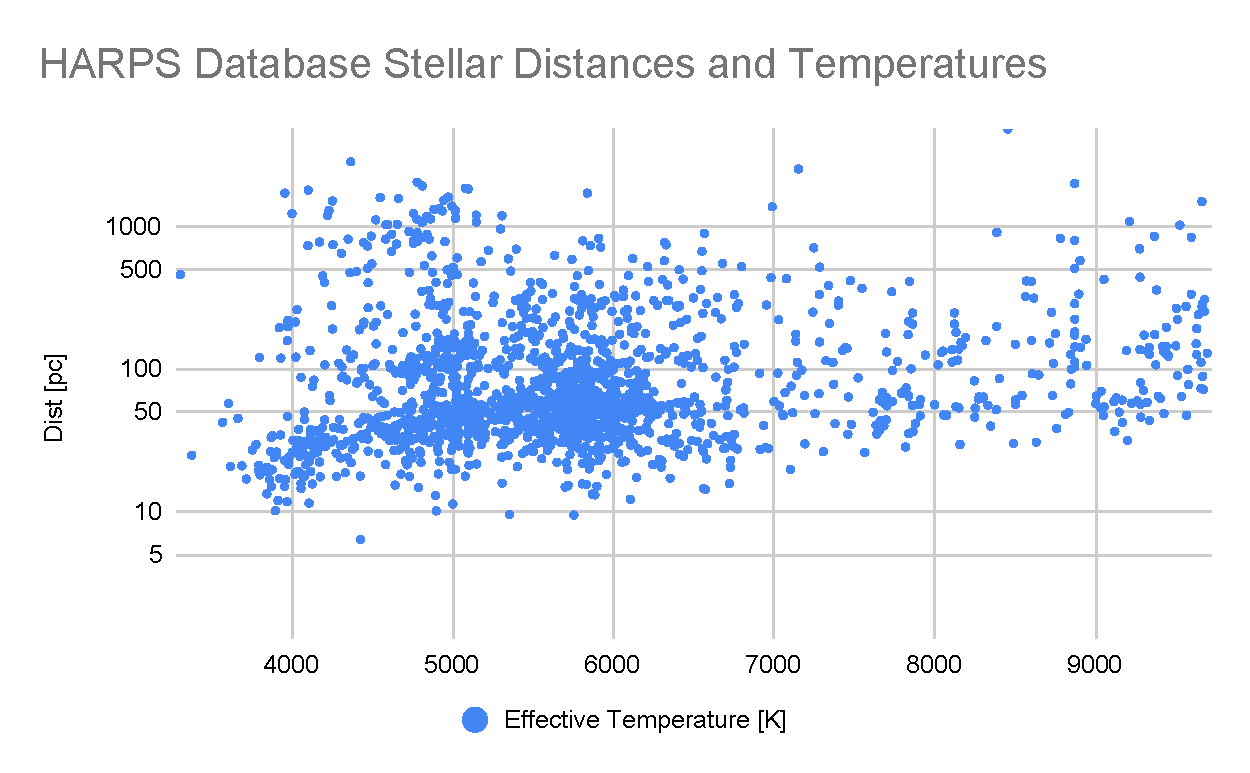
\includegraphics[width=\columnwidth]{harps_database_stellar_distances_and_temperatures.pdf}
    \caption{Temperatures (x-axis, Kelvin) and distances (y-axis, parsecs) of the stellar population targeted by this study. }
    \label{fig:starlist}
\end{figure}

As can be seen in Figure \ref{fig:starlist}, this search covers a wide range of stellar temperatures, with cooler stars of types F, G, K, and M with surface temperatures less than 7000 Kelvin being most common. The vast majority of stars surveyed  are within \DIFaddbegin \DIFadd{a distance of }\DIFaddend 500  \DIFaddbegin \DIFadd{parsec }\DIFaddend or less. Selecting nearby stars is advantageous for both HARPS exoplanet detection and our laser detection project, as it makes faint signals easier to detect. The spectral types confer a similar advantage, as dimmer stars provide less background light that the laser would need to outshine \citep{Howard_2004}.

In the initial search described in this work, we analyzed only one observation from each of these targets (generally, the first one returned by the ESO HARPS data archive search tool at \url{https://archive.eso.org/cms/data-portal.html}. The first observation returned by the ESO database is not necessarily the first observed chronologically, and was found to be indistinguishable from a random sample.) For the handful of stars which yielded compelling candidates from the initial survey, we analyzed all subsequent observations. One goal of this work is to serve as a  \DIFaddbegin \enquote{proof of concept}\DIFaddend , establishing pipelines and procedures and estimating manual workload for a much larger scale search, which will encompass every available stellar spectrum (approximately 212,000) in the HARPS database, as well as its northern hemisphere counterpart HARPS-N \citep{HARPS_N}. For more detailed discussion, see Section \ref{s:future}.

\section{Search Methodology}
We subjected the targets to increasing levels of scrutiny, from automated search tools to detailed manual analysis.  We organized our search by tiers: candidates that pass the Tier 1 tests become Tier 1 candidates, which proceed to Tier 2 analysis, and so on.

The structure of our search is as follows:
\begin{itemize}
    \item Tier 1: Automated Search and Airglow Detection (Section \ref{s:automated})
    \item Tier 2: Manual Assessment of Other False Positives (Section \ref{s:falsepositive})
    \item Tier 3: Curve-Fitting Analysis (Section \ref{s:curvefit})
    \item Interlude: Detailed inspection of the  \DIFaddbegin \DIFadd{HD 127423 }\DIFaddend Candidate (Section  \DIFaddbegin \DIFadd{\ref{s:HD 127423}}\DIFaddend )
    \item Tier 4: Same-Night Doppler Detection of Unknown Terrestrial Sources (Section \ref{s:doppler})
    \item Coda: Searching for Repeat Occurrences (Section \ref{s:repeat})
\end{itemize}

Figure \ref{fig:sankey} in Section \ref{s:results} provides a diagram of the flow of our search strategy, visualized as a Sankey diagram \citep{sankey1898}.

\subsection{Tier  1: Automated Search Algorithm}
\label{s:automated}
Our search algorithm must differentiate between possible laser signals, natural emission lines from the star or Earth's atmosphere, and artifacts created inside the HARPS instrument. We use the spectral width of the feature as one of our distinguishing parameters. The  \DIFaddbegin \DIFadd{line-spread function (LSF}\DIFaddend ) describes the spectral resolution of the instrument, and shows how the instrument's optics would spread out a monochromatic light source to a finite spectral width at the instrument's CCD cameras. The full width half-maximum (FWHM) describes the the observed width of a spectral feature. Since we are searching for near-monochromatic signals emitted from space, we should look for spikes in the spectral data whose FWHM is similar to the instrument's  \DIFaddbegin \DIFadd{LSF}\DIFaddend .

Observed spectral peaks with a FWHM narrower than the  \DIFaddbegin \DIFadd{LSF }\DIFaddend cannot represent light that passed through the instrument's optics, and are likely to be cosmic ray hits or other instrumental artifacts. Conversely, broader spikes  \DIFaddbegin \DIFadd{are difficult to distinguish }\DIFaddend from natural sources whose emission lines are broadened by thermal doppler broadening and other high temperature astrophysical processes. For a more nuanced discussion of broadening mechanisms and their impact on distinguishing artificial signals from natural emissions, see Section \ref{s:stellaremission}.

Our automated search algorithm follows a similar approach to previous archival optical SETI surveys \citep{Tellis_2017,Lipman_2019,Marcy_2021}. First, it establishes a baseline  \DIFaddbegin \enquote{continuum} \DIFaddend stellar flux describing the star's overall spectrum by performing a running median filter with a width of $w$=1000 pixels (10 \DIFaddbegin \DIFadd{~\AA}\DIFaddend ).  This is wide enough to smooth away many natural absorption and emission lines, but narrow enough to minimize the data discarded at the extreme ends of the spectrum. 

Next, it searches for data points that rise beyond a threshold above the running median.  We explored two ways to set the threshold.  The most obvious is just the $w$-point running standard deviation of the spectral data, times a tuneable sensitivity factor $K$.  However, the standard deviation is sensitive to outliers -- such as the spikes we're looking for!  In practice, we found that a standard deviation-based threshold rose dramatically near spectral peaks, making them difficult to detect. (See Figure \ref{fig:threshold}.) Absorption features also distorted the local standard deviation, arbitrarily raising the threshold and also potentially ignoring real spikes in the process.

A better method is to use the $w$-point running 85th percentile.  If the data were normally distributed, the 85th percentile would be one standard deviation above the mean/median, but the 85th percentile is much more robust to outliers such as the spikes we're trying to detect.  A large window width $w$=1000 also gives a more sensitive and consistent threshold.

\begin{figure}
    \centering
    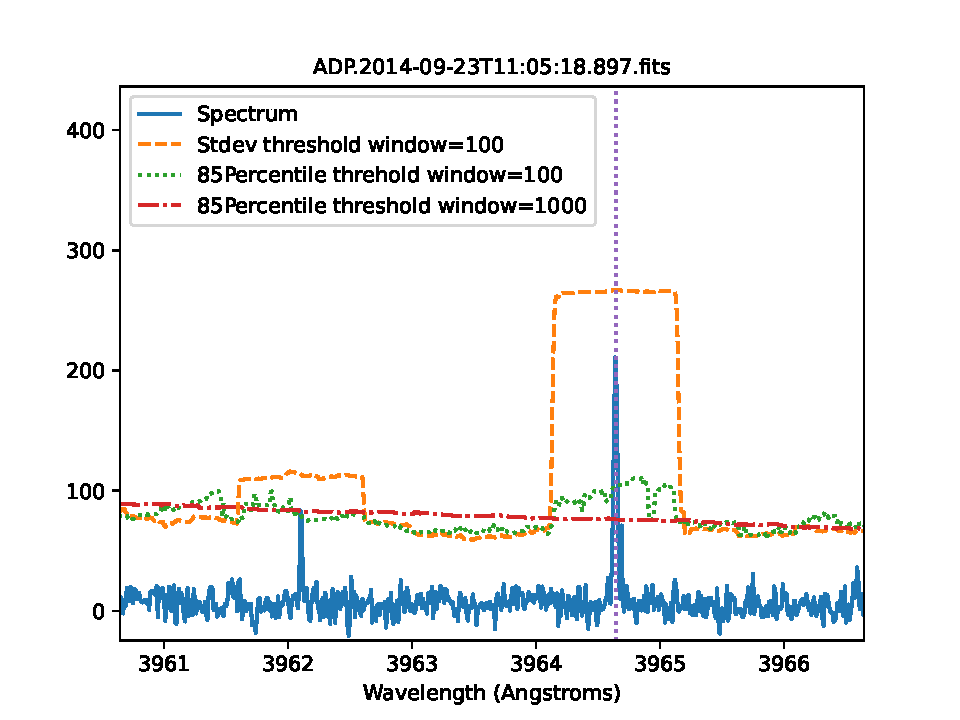
\includegraphics[width=\columnwidth]{threshold.pdf}
    \caption{A comparison of thresholds considered for our automated spike detection algorithm.  Solid blue: part of an example HARPS spectrum.  Dashed orange: spike detection threshold based on running standard deviation with a window width w=100.  This threshold rises near the spikes, so our algorithm would not detect either. Dotted green: threshold based on running 85th percentile with a window width w=100. Note the lower threshold near the spikes.  Dash-dotted red: threshold based on running 85th percentile with a window width w=1000. This gives a low, flat threshold and thus more sensitive and robust spike detection.  Our automated search detects the spike at 3964.6~\AA.  The one on the left has too few points above the detection threshold and would not be flagged.}
    \label{fig:threshold}
\end{figure}

Thus, we look for spikes that rise above the continuum more than $K$=7.5 times the difference between a running 85th percentile and the running median, a relationship  described in the equation below:
\begin{equation}
   T = K (P_{85} -   \DIFaddbegin \DIFadd{P_{50}}\DIFaddend )
   \label{eq:threshold}
\end{equation}
Where $T$ represents the threshold, $P_{85}$ is the running 85th percentile, and $M$ is the the running median. The sensitivity constant $K$ is a tuneable parameter, chosen to be as low as possible to maximize sensitivity, but high enough minimizing the number of false positives that require manual follow-up.  The choice was motivated by a signal injection recovery test (see Section \ref{s:injection_and_recovery}.)

Our algorithm looks for multiple spectral data points in a row that exceed this threshold, within both a minimum and maximum spike width. The HARPS instrument has an average  \DIFaddbegin \DIFadd{line spread function (LSF}\DIFaddend ) of approximately 4.1 pixels \citep{HARPS_specs} or 0.04 \DIFaddbegin \DIFadd{~\AA}\DIFaddend , so monochromatic signals from space should be spread out at least this much. The HARPS  \DIFaddbegin \DIFadd{LSF }\DIFaddend varies by wavelength, but 4 pixels is near the minimum.  Thus, we look for \emph{at least four pixels in a row} at or above 7.5 times the difference between the running 85th percentile and the running median. 

The algorithm also ignores any spikes with more than 500 spectral data points in a row above the threshold. This maximum criterion helps to eliminate natural stellar emission lines, which tend to have wider peaks due to natural spectral line broadening mechanisms (see Section \ref{s:stellaremission}), and prevents spurious  \DIFaddbegin \enquote{detections} \DIFaddend at the edge of the HARPS instrument's inherent data gap. It also allows for lasers which may be broadened beyond the instrumental minimum, whether by heavy modulation or other technological mechanisms. The 1000-point running median filter used to establish the continuum cannot smooth away spectral features wider than about half the filter width, so our algorithm is insensitive to such wide spikes anyway.  Spikes wider than 4 spectral data points above the threshold but narrower than 500 are flagged as initial potential laser candidates and subjected to further review (See Section \ref{s:falsepositive}). 

\subsubsection{Sensitivity  \DIFaddbegin \DIFadd{Testing}\DIFaddend }
\DIFaddbegin 

\DIFadd{In the example in Figure \ref{fig:threshold}, an observation with a very faint continuum was chosen to highlight the differences between search tactics in a noisy spectrum: this figure does not demonstrate the sensitivity limit of our algorithm.  Figure \ref{fig:seti_candidate_CD-312415} later in the text shows that it is sensitive to spikes that rise 10-12\% above the stellar flux, similar to previous work by \cite{Tellis_2017} and others.
}

\DIFaddend We performed a Monte Carlo test to ensure that our spike-detection algorithm was not sensitive to spikes caused by statistical random noise.  If each HARPS spectral data point were an independent Gaussian random variable, the odds that 4 in a row would reach the Eq. \ref{eq:threshold} threshold with $K=7.5$ would be astronomical.  But because of the  \DIFaddbegin \DIFadd{instrument's line-spread function (LSF}\DIFaddend ), adjacent data points are not independent: the lag-1 autocorrelation of a typical HARPS spectrum is about 0.84.  We passed Gaussian white noise through a moving-average filter (window width=6) to create 1000 random synthetic datasets with the same length and lag-1 autocorrelation as typical HARPS data.  Our spike detection algorithm registered zero hits on this synthetic dataset, demonstrating its insensitivity to random noise.

\subsection{Automated Airglow Detection}
\label{s:Airglow}
Atomic transitions in Earth's atmosphere (airglow) are a major source of false positives in our analysis.  Since these emission lines come from heavy atoms in a cool low-pressure atmosphere, their spectral width is near the instrumental  \DIFaddbegin \DIFadd{LSF}\DIFaddend . Therefore, they are difficult to distinguish from lasers using linewidth alone. However, night sky airglow emissions only occur at specific wavelengths--a property which lends itself well to automated filtering.  Care is required regarding doppler shifts and reference frames. The HARPS data processing pipeline shifts the reduced HARPS spectra into the barycentric reference frame by default.  To ensure we are comparing wavelengths in the terrestrial reference frame, we reverse that shift using the Doppler shift equation:
\begin{equation}
    \lambda = \lambda_0 \sqrt{\frac{c + v}{c - v}}
    \label{eq:doppler}
\end{equation}
with $\lambda_0$ and $\lambda$ being the wavelengths in the barycentric and terrestrial frame respectively, $c$ being the speed of light, and $v$ the velocity between frames given by the \texttt{HIERARCH ESO DRS BERV} parameter stored in the FITS header.  

Our automated search tool compares the wavelength (in  \DIFaddbegin \DIFadd{the observatory}\DIFaddend 's reference frame) of each hit returned by our algorithm to wavelengths of known airglow lines, using a comprehensive database of 2,809 night sky emissions compiled in \cite{faint_airglow_database}. The dataset also has the FWHM for each airglow line. In practice, we found that bounding our airglow matching algorithm to a wavelength window 2.5 times the FWHM of each line was effective at rejecting airglow lines while minimizing the total amount of spectrum  \DIFaddbegin \DIFadd{“}\DIFaddend black-listed \DIFaddbegin \DIFadd{” }\DIFaddend by this strategy.  This narrow selection also means that any extraterrestrial laser that used the same atomic transition as an airglow line would probably \emph{not} be falsely categorized as airglow, because it would be doppler-shifted outside the narrow exclusion region. 

For a visual example of an airglow line detected by our automated search tool, see Figure \ref{fig:airglowexample}.

\begin{figure*}
    \centering
    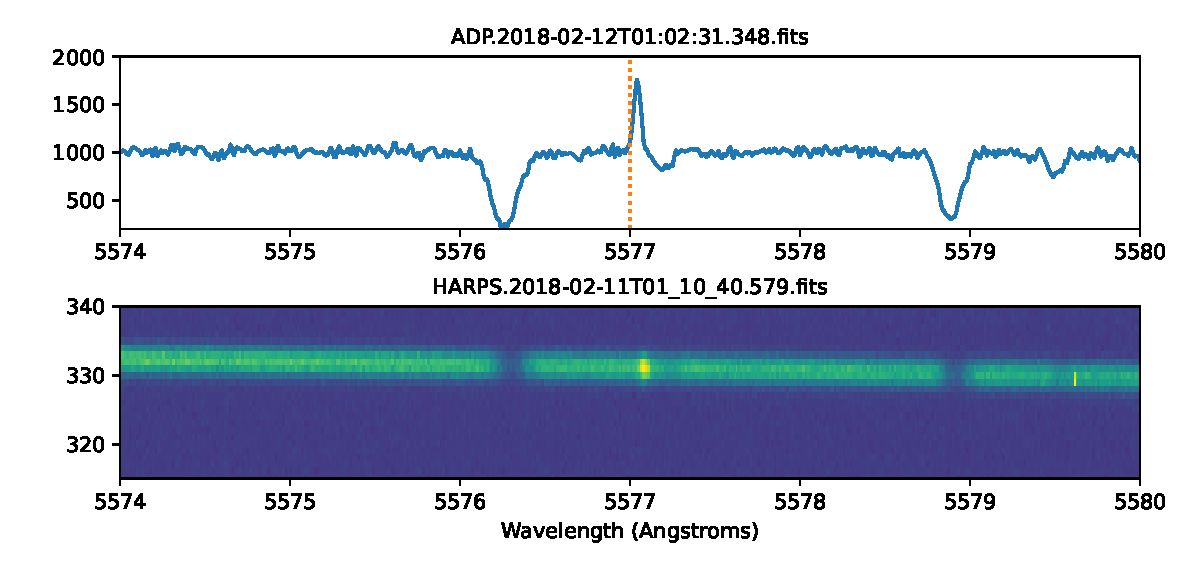
\includegraphics[width=.8\textwidth]{airglowexample.pdf}
    \caption{An example of a commonly recurring airglow line at 5577~\AA\DIFaddbeginFL \DIFaddFL{~}\DIFaddendFL (Observation Date/Time: 2018-02-11, 01:10:40.579). Top panel: reduced spectrum (the red dashed line indicates the spike detected by the automated algorithm). Bottom panel: subsection of the corresponding CCD image for this wavelength range. The stellar spectrum is the  \DIFaddbeginFL \DIFaddFL{green }\DIFaddendFL band. At the location of the detected spike, the CCD image shows a visible corresponding bright spot. Wavelengths  \DIFaddbeginFL \DIFaddFL{in }\DIFaddendFL both the reduced 1-D spectrum and the 2-D CCD image are shown in the  \DIFaddbeginFL \DIFaddFL{terrrestrial (observatory) }\DIFaddendFL reference frame.}
    \label{fig:airglowexample}
\end{figure*}

\subsection{Automated Detection Sensitivity and Power Requirements for Transmitting Lasers}
If one of our candidate signatures came from an extraterrestrial laser, how powerful would it need to be for us to detect it? Our calculation follows \cite{Lipman_2019}.  We do not know the diameter of the aperture of the laser's transmitting optics: in these calculations, we assume  \DIFaddbegin \DIFadd{a 5~m diameter}\DIFaddend .

The laser beam will spread out by diffraction as it travels to Earth, with an opening angle:

\begin{equation}
    \theta = \frac{1.22\lambda}{d_T}
\end{equation}
where $\lambda$ is the wavelength of the beam and $d_T$ the diameter of the transmitter's aperture.  On reaching Earth, the beam will spread out into a disk of area:

\begin{equation}
    A = \pi r^2 = \pi ( \DIFaddbegin \DIFadd{\frac{\theta}{2} }\DIFaddend D)^2 = \pi  \DIFaddbegin \DIFadd{\frac{1.22^2 \lambda^2 D^2}{4d_T^2}
}\DIFaddend \end{equation}
where $D$ is the distance from the transmitter to Earth.  If the transmitting laser's luminosity is $L_T$, the luminous flux at Earth is

\begin{equation}
    F = \frac{L_T}{A} =  \DIFaddbegin \DIFadd{\frac{4L_T d_T^2}{\pi 1.22^2 \lambda^2D^2}
}\DIFaddend \end{equation}
The power, in watts, entering the receiving telescope is thus

\begin{equation}
    P_R = A_R F = \pi (d_R/2)^2 F =  \DIFaddbegin \DIFadd{\frac{4L_T d_T^2 d_R^2}{1.22^2 \lambda^2 D^2}
}\DIFaddend \end{equation}
where $A_R$ is the area and $d_R$ the diameter of the receiving telescope.   \DIFaddbegin \DIFadd{Since the energy per photon is $E_p = h c / \lambda$, the }\DIFaddend number of photons entering the telescope over the course of an observation of duration $T$ is thus

\begin{equation}
    N =  \DIFaddbegin \DIFadd{\frac{P_R T}{E_p} }\DIFaddend =  \DIFaddbegin \DIFadd{\frac{4L_Td_T^2 d_R^2 T}{1.22^2 \lambda h c D^2}
}\DIFaddend \end{equation}
where $h$ and $c$ are Planck's constant and the speed of light.  Accounting for the instrument's quantum efficiency $\epsilon$, the number detected will be
\begin{equation}
    \label{eq:transpower}
    N_{\mbox{det}} =  \DIFaddbegin \DIFadd{\frac{4\epsilon L_T d_T^2 d_R^2 T}{1.22^2 \lambda h c D^2}
}\DIFaddend \end{equation}
Solving for the transmitter power $L_T$:
\begin{equation}
    L_T =  \DIFaddbegin \DIFadd{\frac{1.22^2 N_{\mbox{det}} \lambda h c D^2}{4\epsilon d_T^2 d_R^2 T}
}\DIFaddend \end{equation}

For the purposes of this analysis, we assume the laser is powered on for the duration of the exposure time. If the transmitter were pulsed, higher power would be needed, in proportion to the transmitter's duty cycle. 

This calculation does not factor in extinction due to interstellar dust.  \cite{Hippke_2018} estimated power losses due to astronomical dust,  \DIFaddbegin \DIFadd{quantifying it as $S_E$, or the fraction of photons received across a given interstellar distance. According to \citep{Hippke_2018} becomes a relevant factor ($S_E< 0.5$)  at }\DIFaddend distances $>=$ 300 pc. Since a majority of HARPS stellar targets are within 250 pc, we treat this as insignificant.

We use the derivation above to establish minimum detectable power in the following section.

\subsection{Injection/Recovery Test}
\label{s:injection_and_recovery}
To assess the sensitivity of our search algorithm, we injected artificial laser-like Gaussian spikes into spectral data from HARPS. We started with single HARPS observations of 20 stars, of spectral
types F,G,K and M, at distances between 3 and 170 \DIFaddbegin \DIFadd{~pc}\DIFaddend . We ensured that these observations were devoid of spikes before injecting our artificial signals.  For each of them, we added an
artificial Gaussian spike at a random wavelength, with a FWHM equal to the HARPS spectral
resolution at that wavelength, and a peak flux (calculated using Eq. \ref{eq:transpower}) corresponding to a random laser power between 500 W and 10 MW and a nominal transmitter aperture of  \DIFaddbegin \DIFadd{5~m}\DIFaddend . We then checked to see if our search algorithm recovered this artificial signal. For each of the 20 stars, we repeated this process 100 times each with random laser powers in five ranges (500 W-1 kW), (1 kW-10 kW), (10 kW-100 kW), (100 kW-1 MW), (1 MW-10 MW). This constituted 500 injections per observation/star, totaling 10,000 separate injection and recoveries across the entire analysis. To ensure uniform wavelength coverage, each set of 100 injections consisted of 50 injected lasers with random wavelengths covering the shorter portion of HARPS' spectral range (3995.00~\AA-5423.19~\AA), and 50 covering the longer portion of HARPS' wavelength range (5423.19\DIFaddbegin \DIFadd{~}\DIFaddend \AA-6850.69\DIFaddbegin \DIFadd{~}\DIFaddend \AA).

\DIFaddbegin \DIFadd{We perform our injection analysis on processed spectra rather than raw CCD images.  To test whether de-blazing and other pipeline steps cause the flux values in the processed spectra to differ from the raw number of quanta detected by the CCD, we compared the integrated flux values in a small region of a handful of raw CCD images against the same region in their processed spectra.  We found that the processing steps change the integrated count values by only -15/+30\% near the center/edge of a typical HARPS CCD image.  Thus we are justified in using the processed spectra for this order-of-magnitude injection test. 
}

\DIFaddend \begin{figure*}
    \centering   \DIFaddbeginFL 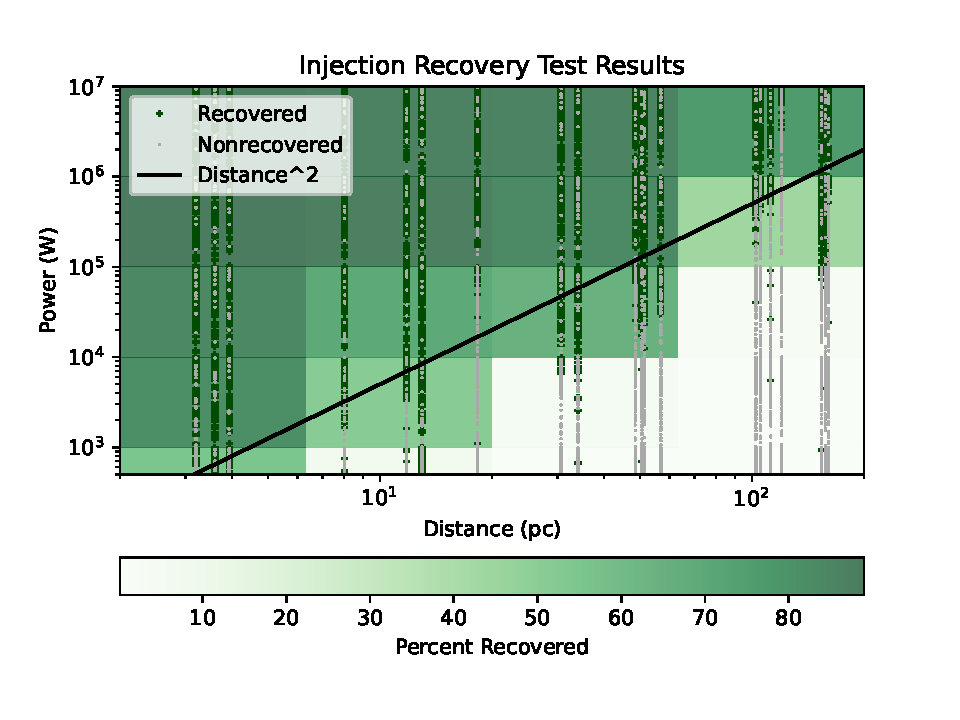
\includegraphics[width=.8\textwidth]{injection_recovery_gridded.pdf}
    \DIFaddendFL \caption{Results of our  \DIFaddbeginFL \DIFaddFL{signal }\DIFaddendFL injection/recovery test. Each dot represents an artificial laser-like spike with a randomly-chosen laser power, injected into HARPS spectra of stars of various types and distances.   \DIFaddbeginFL \DIFaddFL{Green crosses }\DIFaddendFL indicate \DIFaddbeginFL \DIFaddFL{that }\DIFaddendFL the artificial signal was recovered by our algorithm, while  \DIFaddbeginFL \DIFaddFL{grey }\DIFaddendFL dots indicate a null detection. The \DIFaddbeginFL \DIFaddFL{color of the shaded boxes indicates the percentage of injected signals recovered within that box.  The }\DIFaddendFL black diagonal line represents the slope of an inverse square law, correlating closely to signal recovery as a function of distance.}
    \label{fig:injection_recovery_results}
\end{figure*}

Figure \ref{fig:injection_recovery_results} shows that the vast majority of artificial injected signals are recovered by our search algorithm at high laser power or short distances. As expected, injected signals with low amplitude (large distance, small power) are difficult to detect. The detection threshold is not far from an inverse square law, though the threshold also varies from star to star.  

Quantitatively, we found that we can detect injected signals with simulated powers of 500 Watts - 1 Kilowatt under 10  \DIFaddbegin \DIFadd{pc}\DIFaddend , with a recovery rate of almost 90\%. At between 10 and 100  \DIFaddbegin \DIFadd{pc}\DIFaddend , the required input power ranges from 10-100 kilowatts. At a distance of  100 \DIFaddbegin \DIFadd{~pc }\DIFaddend or more, lasers need  \DIFaddbegin \DIFadd{$\sim$ }\DIFaddend 1 MW or greater of brightness to be detectable.  \DIFaddbegin \DIFadd{Distance is not the only factor: detectability does vary between stars of different distances.  However, the }\DIFaddend recovery rate showed no obvious dependence on the spectral type of the background star. There was also no observable wavelength bias, indicating our algorithm could effectively recover lasers across the entire spectrum.

For most targets in this survey, our method is sensitive enough to detect lasers that could be built with current human technology \citep{Lander1997ContinuouswaveCD}.


\subsection{Tier 2: Eliminating Other False Positives}
\label{s:falsepositive}
Our Tier 1 automated search, based on the above criteria (4-500 pixels in a row above threshold, with airglow lines excluded) yielded 508  \DIFaddbegin \enquote{spike} \DIFaddend candidates from our 2,821 stars. Additional manual analysis was performed to exclude other false positives.

In Tier 2, we visually inspected the CCD images of each of these 508 observations to identify potential false positives and distinguish potential technosignatures from prosaic phenomena.  In addition to airglow lines (considered in Tier 1 (Section \ref{s:Airglow}), we looked for three other categories of false positive: cosmic rays, stellar emission lines, as well as instrumental effects.

\subsubsection{Overlapping Order Test}
\label{s:overlapping_orders}
HARPS's echelle spectrograph design provides a useful way to identify spectral features that originate from inside the instrument rather than the target.  Each of HARPS's 72 spectral orders covers a different portion of the overall wavelength range. These ranges partially overlap at the ends, so some wavelengths are found in two orders.  If a real `extra-instrumental' light source has a wavelength in the overlap range, it will produce \emph{two} bright spots on the CCD image, one in each spectral order. Therefore, if we see a bright spot that occurs in only one order but not in the other overlapping one, this strongly indicates a cosmic ray hit, instrumental artifact, or other intra-instrumental source.  Conversely, if the bright spots show up in both relevant spectral orders, we can rule out these types of  \DIFaddbegin \DIFadd{false positives}\DIFaddend .

Therefore, if a spike is found in an  \DIFaddbegin \enquote{order overlap region}\DIFaddend , our CCD visualization tool shows both orders, streamlining detection of artifacts.  However, this method only  \DIFaddbegin \DIFadd{applies  }\DIFaddend where the spike is found in the overlap regions, which amount to about 20\% of the spectrum.  This method allowed us to significantly improve manual detection of false positives in these cases.  An example is shown in Figure \ref{fig:Cosmic_ray_example} and discussed below.

\subsubsection{Cosmic Rays}
\label{s:cosmic}
Cosmic rays can collide with the HARPS instrument's CCD sensors, scattering electrons and creating false  \DIFaddbegin \enquote{spikes}\DIFaddend . Since these spikes are not created by light passing through the instrument, many will be narrower than the instrument's  \DIFaddbegin \DIFadd{LSF}\DIFaddend , and will be filtered out by the algorithm's  \DIFaddbegin \enquote{4-in-a-row} \DIFaddend criterion.  However, in some cases high-energy particles can slice through multiple pixels at an angle, forming meteor-like tracks in the raw CCD image and creating a spectral peak more than 4 pixels wide.  To detect such cases, we manually inspected the raw CCD images for each automatically-detected peak to visually identify patterns characteristic of cosmic rays, utilizing a methodology similar to \cite{Tellis_2017}. 

We identified likely cosmic rays by visual inspection using the following criteria:
\begin{enumerate}
    \item a long, narrow track on the CCD image that was not aligned with the spectrometer's entry slit, or
    \item a CCD signal that spills over into parts of the image that are not illuminated by the starlight passing through the spectrometer's entry fiber, or
    \item a signal that does not fully occupy the width of the region illuminated by the entry slit.
\end{enumerate}
We manually classified a detection as a  \DIFaddbegin \enquote{likely cosmic ray} \DIFaddend if it had any of these features, using the overlapping order test (Section \ref{s:overlapping_orders}) to corroborate when possible.

Figure \ref{fig:Cosmic_ray_example} shows an example of a cosmic ray detection, as indicated by both track shape and the multi-order test.

\begin{figure*}
    \centering
    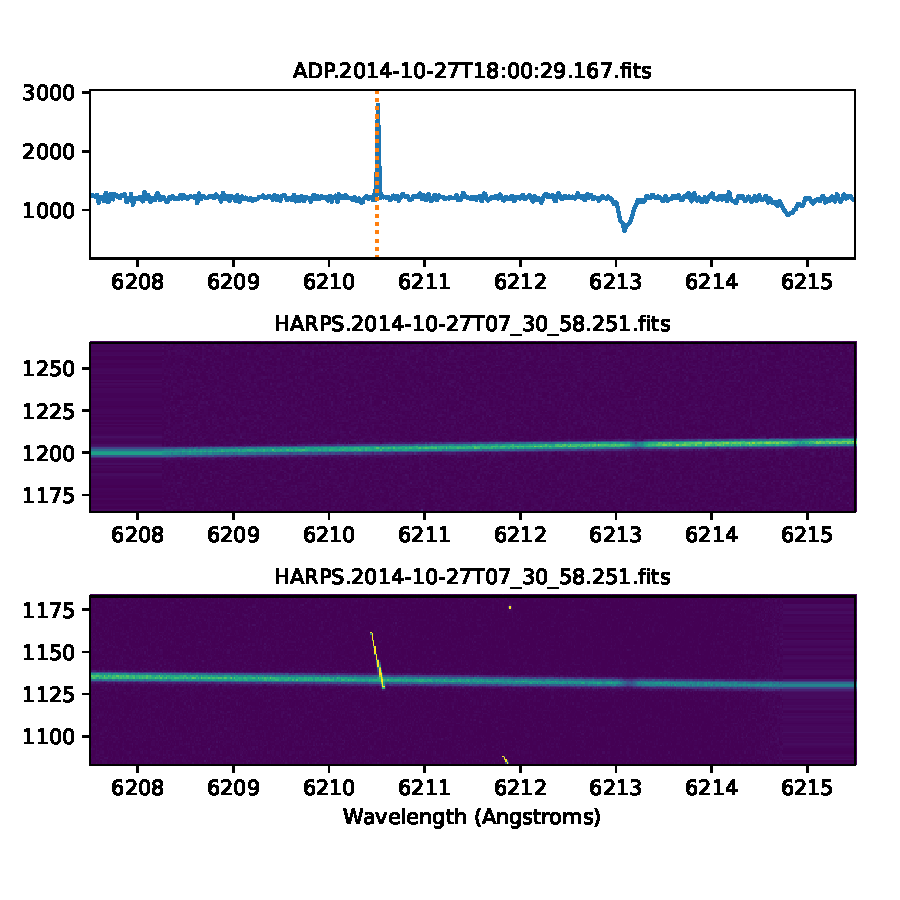
\includegraphics[width=.8\textwidth]{Cosmic_ray_multiorder_example.pdf}
    \caption{An example of a cosmic ray detection (Observation Date/Time: 2014-10-27, 07:30:58.251). Top panel: reduced spectrum (the red dashed line indicates the spike detected by the automated algorithm).  In this case, the target wavelength appears in two different spectral orders of the HARPS echelle spectrograph: the two regions of the CCD image containing the target wavelength are shown in the middle and lower panel.  The stellar spectrum is the pale blue band. In the bottom panel, the CCD image shows a long track which spills over outside the band of starlight on the image.  This track is not present in the middle panel. These two lines of evidence each show that the spike was caused by a cosmic ray striking the CCD, and not light from the target. \DIFaddbeginFL \DIFaddFL{Wavelengths in both the reduced 1-D spectrum and the 2-D CCD image are shown in the terrrestrial (observatory) reference frame.}\DIFaddendFL }  
    \label{fig:Cosmic_ray_example}
\end{figure*}

\subsubsection{Instrumental Effects}
\label{s:bleedthrough}
 The HARPS instrument contains a Th-Ar calibration lamp, an artificial reference spectrum imaged in the same CCD frame as the stellar spectrum to calibrate the wavelengths being measured \citep{HARPS_specs}. In some observations, the calibration lamp was left on during the observation, either deliberately or by mistake.  This led to another class of false positives,  \DIFaddbegin \enquote{calibration lamp bleed-through} \DIFaddend (see Figure \ref{fig:bleedthrough}).

\begin{figure*}
    \centering
    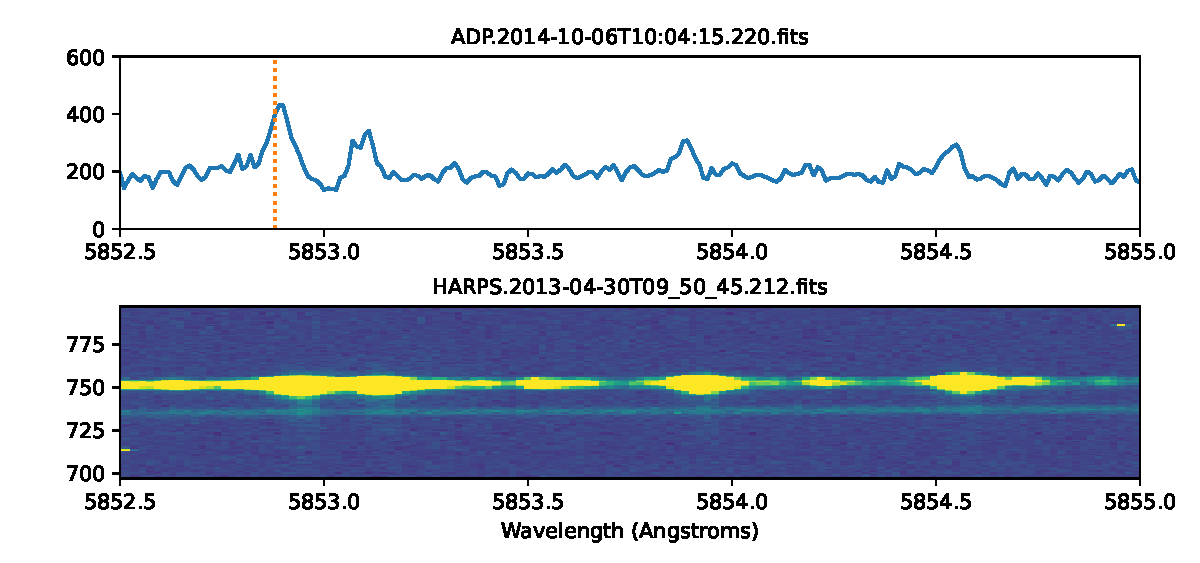
\includegraphics[width=.8\textwidth]{bleedthrough.pdf}
    \caption{An example of calibration lamp bleed-through (Observation Date/Time: 2013-04-30, 09:50:45.212). Top panel: reduced spectrum, bottom panel: raw CCD image. The upper band of bright spots in the CCD image is from the calibration lamp; the lower band is starlight.  Charge from an oversaturated emission line in the calibration lamp has bled across to contaminate the stellar spectrum. \DIFaddbeginFL \DIFaddFL{Wavelengths in both the reduced 1-D spectrum and the 2-D CCD image are shown in the terrrestrial (observatory) reference frame.}\DIFaddendFL }
    \label{fig:bleedthrough}
\end{figure*}

In the example shown in  \DIFaddbegin \DIFadd{\ref{fig:bleedthrough}}\DIFaddend , the calibration lamp's bright spectral peaks (seen in the upper part of the CCD image)  \DIFaddbegin \DIFadd{“bleed through” }\DIFaddend vertically, creating a spurious spike in the stellar spectrum below.  Since the width of these spikes is close to the instrument's  \DIFaddbegin \DIFadd{LSF}\DIFaddend , this category of false positive cannot be identified automatically in processed spectra and was identified by manual inspection of the CCD images.

Additionally, we noted another likely instrumental artifact--a series of closely clustered spikes, similar in profile to  \DIFaddbegin \DIFadd{“combs” }\DIFaddend first observed in \citep{ProximaCentauri}. In his analysis, \citeauthor{ProximaCentauri} hypothesized that glass in the HARPS apparatus creates internal reflections yielding interference patterns similar in effect to a Fabry-Perot etalon. We observed similar interference fringes, with a recurrent wavelength range (around 3852~\AA) across numerous observations, identical in profile to the ones noted in \citep{ProximaCentauri} (albeit at a different set of wavelengths). We visually identified these artifacts and excluded them from further consideration. For an example of such interference fringes, see Figure \ref{fig:interferencepattern}.

\begin{figure*}
    \centering
    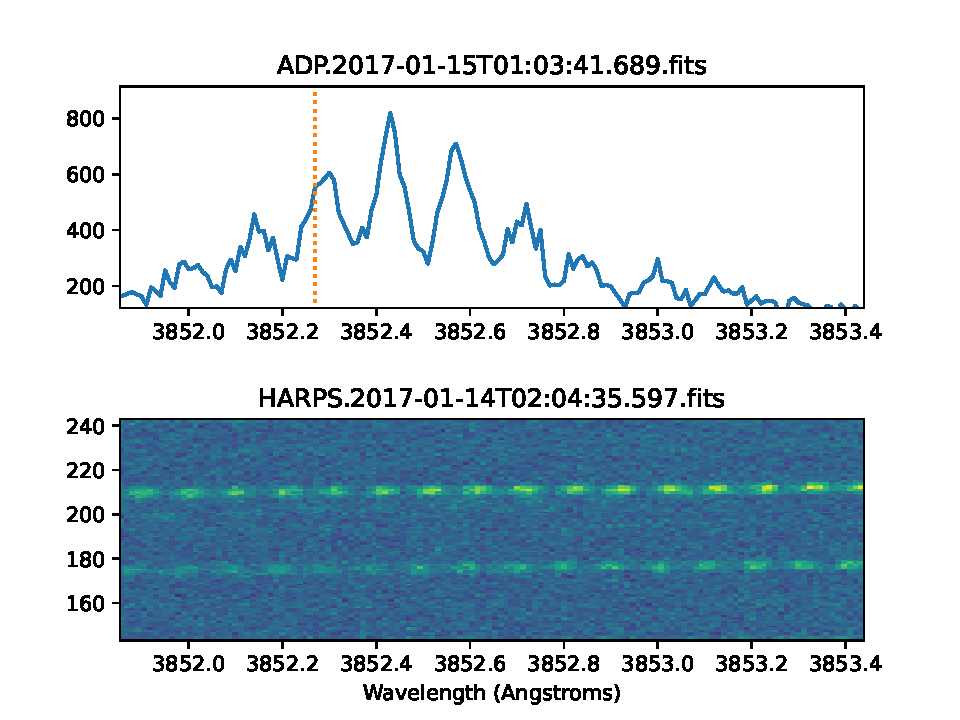
\includegraphics[width=0.8\textwidth]{etalonfringesexampleforpaper.pdf}
    \caption{An example of a recurrent instrumental artifact, possibly indicative of internal reflections forming an interference pattern (Observation Date/Time: 2017-01-14, 02:04:35.597). Top panel: reduced spectrum, bottom panel: raw CCD image. \DIFaddbeginFL \DIFaddFL{Wavelengths in both the reduced 1-D spectrum and the 2-D CCD image are shown in the terrrestrial (observatory) reference frame.}\DIFaddendFL }
    \label{fig:interferencepattern}
\end{figure*}
\DIFaddbegin 

\DIFaddend In a few cases, the multi-order test outlined in \ref{s:overlapping_orders}) revealed bright spots appearing on one order and not the other, but which did not meet the visual criteria for cosmic rays outlined in Section \ref{s:cosmic}.  We categorized these as likely instrumental artifacts, because any real  \DIFaddbegin \DIFadd{“}\DIFaddend extra-instrumental light \DIFaddbegin \DIFadd{” }\DIFaddend that falls within a wavelength range imaged by two spectral orders should appear in both parts of the CCD image, not just one.

\subsubsection{Natural Stellar Emission Lines}
\label{s:stellaremission}
Natural emission lines from stars could also be detected by our spike-searching algorithm.  These natural sources have two features that might distinguish them from lasers. First, due to thermal doppler broadening, emission lines from hot low-molecular-weight gases tend to have spectral peaks much broader than the HARPS instrument's  \DIFaddbegin \DIFadd{LSF}\DIFaddend . However, emission lines from cooler stars, or those from heavier elements, may be narrower \citep{Livadiotis_2018}. Natural stellar emission lines also undergo broadening from other mechanisms, including pressure/collisional \citep{Peach2006} and rotational \citep{Rotational_Broadening}. All of these mechanisms can make natural stellar emission lines appear noticeably broader than a laser would. 

Second, natural stellar emission lines rarely show up in isolation. Most stars do not have strong emission lines; the  \DIFaddbegin \enquote{active} \DIFaddend stars that do tend to have many of them. Typically, a stellar emission line will occur as part of a “series” in which many different atomic transitions of one or more elements are excited in the atmosphere of an active star.  Thus, the number of spectral peaks is another criterion that can distinguish between natural stellar emission lines and lasers. 

We flagged cases  where four or more spikes were detected in a single observation as likelier to be stellar emission features, and subjected them to additional review. Of course, an alien technological source might use multiple laser wavelengths--however, it remains a telltale characteristic of natural stellar activity \citep{Livadiotis_2018}, especially when coupled with relatively wide peaks due to the thermal doppler broadening that the heat of a star would likely produce and coming from a spectral type or star which is already known to be chromospherically active. Regarding the doppler broadening, there can be exceptions.  \DIFaddbegin \DIFadd{In a previous HARPS study of Proxima Centauri, \citep{ProximaCentauri} found hundreds of narrow emission lines from heavy elements, with narrow linewidths around .06 \AA. \cite{ProximaCentauri} notes that these narrow emission lines were associated with flaring events, which demonstrates that under the right conditions }\DIFaddend some M-type stars  \DIFaddbegin \DIFadd{can produce narrow, nearly `}\DIFaddend laser-like'  \DIFaddbegin \DIFadd{emission lines}\DIFaddend . However, in such cases the flaring activity will produce a multitude of emission lines and any spikes will not appear in isolation.

For an example of a spectrum which matches our criteria for natural stellar emission lines, see Figure \ref{fig:eruptivevariablestar} from eruptive variable star  \DIFaddbegin \DIFadd{GJ 234.
}\DIFaddend 

 \DIFaddbegin \begin{figure*}
    \DIFaddendFL \centering
      \DIFaddbeginFL \begin{overpic}[width=.8\textwidth]{eruptivevariablestar.pdf}
     \put(48,30){\textcolor{red}{Star: GJ 234}}
    \end{overpic}
    \DIFaddendFL \caption{Reduced spectrum of an eruptive variable star,  \DIFaddbeginFL \DIFaddFL{GJ 234. }\DIFaddendFL Numerous spikes are visible, as is typical of natural stellar emission-line activity from eruptive stars like this one.  Inset: Zoom-in on one of approximately 10 spikes observed from this star. These emission features are much broader than the HARPS instrument's  \DIFaddbeginFL \DIFaddFL{line-spread }\DIFaddendFL function, as is typical of natural stellar emission lines.  \DIFaddbeginFL \DIFaddFL{Wavelengths in both the reduced 1-D spectrum and the 2-D CCD image are shown in the terrrestrial (observatory) reference frame}\DIFaddendFL .\DIFaddbeginFL }
    \DIFaddendFL \label{fig:eruptivevariablestar}
 \DIFaddbeginFL \end{figure*}
\DIFaddend 

Of all stellar emission lines observed in this survey, Calcium-II H and K lines (3933~\AA~and 3968~\AA) were by far the most prevalent, with 275 detections in our search. Given how common they were even for stellar types which are otherwise not known for emission lines, we used an automated filter to identify them. Similar to the airglow line detector (Section \ref{s:Airglow}), it uses the known stellar radial velocity \DIFaddbegin \DIFadd{(relative to solar barycenter) }\DIFaddend contained in the observation's \texttt{HIERARCH ESO TEL TARG RADVEL} header to Doppler-shift the observation into the star's reference frame  using Eq. \ref{eq:doppler} and compares it to the known wavelengths of the \DIFaddbegin \DIFadd{Calcium }\DIFaddend H and K lines.

For more complex clusters of spikes (ie, four or more spikes in one spectrum), we categorize the spikes as likely stellar emission if they come from a stellar type where emission lines are common--especially if denoted with a subscript  \DIFaddbegin \enquote{e} \DIFaddend which is generally used to denote emission line stars. Several M-Dwarf stars with clustered hits are also placed in this category, due M-dwarf's propensity for flaring and complex chromospheric behavior \citep{ProximaCentauri}. Two more exotic stars with characteristics indicative of possible emission activity were also included in this category.  \DIFaddbegin \DIFadd{HD 90177 }\DIFaddend is a Luminous Blue Variable star \citep{LBV2}, which are known to produce emission lines \citep{LBV}. CD-332771 is a K-type star in a close eclipsing binary system \citep{CD332771EmissionLinesEclipsingBinaries}. Such eccentric eclipsing binary systems are known for emission activity due to shared envelopes of material and interactions between the two stars \citep{eclipsing_binaries}. The emission line stars in question, along with the total number of initial spikes from each, are listed in Appendix \ref{s:confirmedstellaremissionclusters}.

Any observations containing 4 or more spikes in a row which did \textbf{not} originate from spectral types known to produce emission lines were flagged as a viable candidate, and subjected to the same followup investigation as the rest. 

Manual inspection of CCD frames let us categorize 414 of our candidates as cosmic rays, 13 as calibration lamp bleedthrough, and 17 as other instrumental artifacts.  275 were eliminated as \DIFaddbegin \DIFadd{Calcium }\DIFaddend H and K lines, 27 were manually identified as other common emission lines, and 135 appeared in complex clusters of spikes originating from emission-type stars.  6 observations had too low a signal-to-noise ratio to be manually categorized.  This left us with 64 Tier 2 candidates still unexplained.

\subsection{Tier 3:  \DIFaddbegin \DIFadd{Curve fitting }\DIFaddend algorithm}
\label{s:curvefit}

Although our manual search was effective at spotting many cosmic rays, some will create trails that do not show diagonal streaks or extend outside the stellar spectrum, and will thus not be visually distinctive.  Other unidentified instrumental artifacts might also create false positives.  To rule these out, our Tier 3 analysis fit a Gaussian curve to each of our candidate spikes, and considered its linewidth.  Line features caused by light passing through the HARPS optics will always have a line width greater than the instrument's  \DIFaddbegin \DIFadd{line-spread function (LSF}\DIFaddend ), while cosmic rays or internal artifacts may not. Although we attempted to mitigate this by setting a minimum number of pixels above the threshold in our initial search algorithm (See \ref{s:automated}), the  \DIFaddbegin \DIFadd{LSF }\DIFaddend varies by wavelength and more precise methods are needed to accurately ascertain linewidth.

HARPS has a resolving power of 115000 \citep{HARPS_specs}, meaning that the instrument's  \DIFaddbegin \DIFadd{LSF }\DIFaddend at a given wavelength is: 

\begin{equation}
    \delta\lambda = \frac{\lambda}{115000}
     \DIFaddbegin \label{eq:LSF}
\DIFaddend \end{equation}

We used \texttt{scipy.optimize.curve\_fit()} \citep{2020SciPy-NMeth} to fit a Gaussian curve plus a constant continuum (Eq. \ref{eq:fit}) to each of the 41 remaining candidate spikes and estimated the spike's Full-Width Half-Maximum (FWHM). 

\begin{equation}
    y(\lambda) = A e^{\left(- \frac{\lambda - \lambda_0}{2 \sigma}\right)^2}+y_0
    \label{eq:fit}
\end{equation}

To ensure the curve-fitting tool fit a Gaussian to our spike and not to the continuum or other spectral features, we took the following steps.  First, we fit a Gaussian curve \emph{plus a constant} \DIFaddbegin \DIFadd{. This is to ensure that the Gaussian curve fit measures the excess flux and not the continuum, by raising the baseline to the continuum's level. To ensure that the continuum constant $y_0$ accurately represented the continuum, we required that it lie within the minimum and maximum range of the data in the fitting window, with the midpoint as an initial guess}\DIFaddend . We required that the central wavelength $\lambda_0$ of the Gaussian fit lie within this data window, using the central wavelength of our detected spike as an initial guess. We  \DIFaddbegin \DIFadd{then clipped the data to a window within $\pm$1~\AA~of the center of our detected spike. The 1~\AA~window was chosen to be sufficiently wide to accurately represent the continuum, without allowing in an overabundance of other spikes and absorption features which could confuse it. %DIF > Note to Jason: This can prob be worded better. Have at it!
}\DIFaddend We required that the amplitude $A$ of the Gaussian be positive, using the range of the windowed data as an initial guess. \DIFaddbegin \DIFadd{The positive amplitude requirement ensures that the curve fits exclusively to the candidate spike, and not any nearby absorption features. }\DIFaddend Finally, we required that the width $\sigma$ of the Gaussian be between zero and 1/2 the width of the data window, using 1/6 of the width of the data window as an initial guess.  \DIFaddbegin \DIFadd{This initial guess is somewhat wider than the narrow features we are trying to fit: this improves convergence of the curve-fitting algorithm by casting a wider net to find the spike.
}\DIFaddend 

The algorithm uses a  \DIFaddbegin \enquote{goodness of fit} \DIFaddend parameter and multiple successive fits to converge on an accurate linewidth fit. Ideally, if the best-fit width of a spike is greater than or equal to the instrument's  \DIFaddbegin \DIFadd{LSF}\DIFaddend , the candidate is likelier to be a genuine SETI detection. Otherwise, the candidate signal possibly originates from within the instrument and is therefore likelier to be a cosmic ray or instrumental artifact. In practice, instrumental noise and nearby absorption features add uncertainty and possible bias to the best-fit linewidth, so a strict cut-off at the instrument's  \DIFaddbegin \DIFadd{LSF }\DIFaddend could lead to false categorizations.

We accounted for this by comparing Gaussian curve-fitting statistics for three categories of spikes: 
\begin{enumerate}
    \item Tier 1 candidates which were identified as cosmic rays in our manual inspection.  These should often have line widths below the instrument's FWHM, providing a negative control.  However, sometimes the cosmic ray particles will slice through multiple pixels, thus appearing wider than instrumental  \DIFaddbegin \DIFadd{LSF}\DIFaddend .
    \item Airglow lines identified by our automated search tool.  Since airglow lines originate from cool, heavy atoms, they have line widths near  the instrument's  \DIFaddbegin \DIFadd{LSF}\DIFaddend , and therefore serve as good approximations of laser-like  signals. These constitute a positive control.
    \item Simulated spikes which we injected into the 1-D spectra using the same technique as \ref{s:injection_and_recovery}.  These injected signals have known Gaussian line widths that can be compared to the output of our curve-fitting algorithm.  We only fed injected spikes into the curve fitting algorithm that were strong enough to be successfully recovered by our Tier 1 search tool. 
\end{enumerate}

We used these populations to establish a margin of error for our line width criterion -- a difference between the measured FWHM and the FWHM predicted by  \DIFaddbegin \DIFadd{Equation \ref{eq:LSF} }\DIFaddend over which a majority of  \DIFaddbegin \enquote{real} \DIFaddend spikes and airglow lines would be accepted, while below which sufficiently narrow cosmic rays would be rejected.

Of 339 spikes manually identified as cosmic rays, 243 (72\%) had best-fit line widths below the instrument's  \DIFaddbegin \DIFadd{LSF}\DIFaddend .  Of 1,204 spikes matching the wavelengths of airglow lines, 211 (18\%) had best-fit line widths below the predicted FWHM, with the rest exceeding it.  Of the 4,699 injected gaussian spikes, 1,604 (34\%) had best-fit line widths below the predicted FWHM.  Since a considerable number of airglow lines and injected Gaussians -- our positive controls -- had best-fit FWHMs that fell below the  \DIFaddbegin \DIFadd{LSF}\DIFaddend , a less strict cutoff is needed, one that includes a margin of error.  We observed that only 1.5\% of the injected Gaussian signals had a best-fit FWHM  that was less than the true injected FWHM minus 0.003~\AA.  

Thus, we chose a line width criterion that includes a margin of error.  A spike passes our line width test if it satisfies:
\begin{equation}
    \mbox{Best-Fit FWHM} >  \DIFaddbegin \DIFadd{\mbox{Instrument LSF} }\DIFaddend - 0.003 \mbox{~\AA}
    \label{eq:linewidth}
\end{equation}
With this criterion, the false  \DIFaddbegin \DIFadd{negative }\DIFaddend rate for injected Gaussian spikes drops from 34\% to 1.5\%, and for airglow lines it drops from 18\% to 13\%.   

 With this criterion, the curve-fitting test correctly identifies the vast majority of injected spikes as  \DIFaddbegin \enquote{extra-instrumental}\DIFaddend , and the majority of cosmic ray spikes as  \DIFaddbegin \enquote{intra-instrumental}\DIFaddend , but it should not be considered definitive.  We use it as a criterion to identify candidates which should be given higher priority, but not  one which definitively rules them out. The vast majority of our candidates that fail this final test are likely to be cosmic rays due to how we constructed our test and margin for error, but there may still be a small handful which are `extra-instrumental' sources distorted by instrumental noise. The Tier 2 candidates sifted out during Tier 3 analysis (because their best-fit linewidth was below the criterion in Eq. \ref{eq:linewidth}) are listed in Appendix \ref{s:rejects}.

\section{Results of Tier  \DIFaddbegin \DIFadd{1--3 }\DIFaddend Search}
\label{s:results}

\begin{figure*}
    \centering
    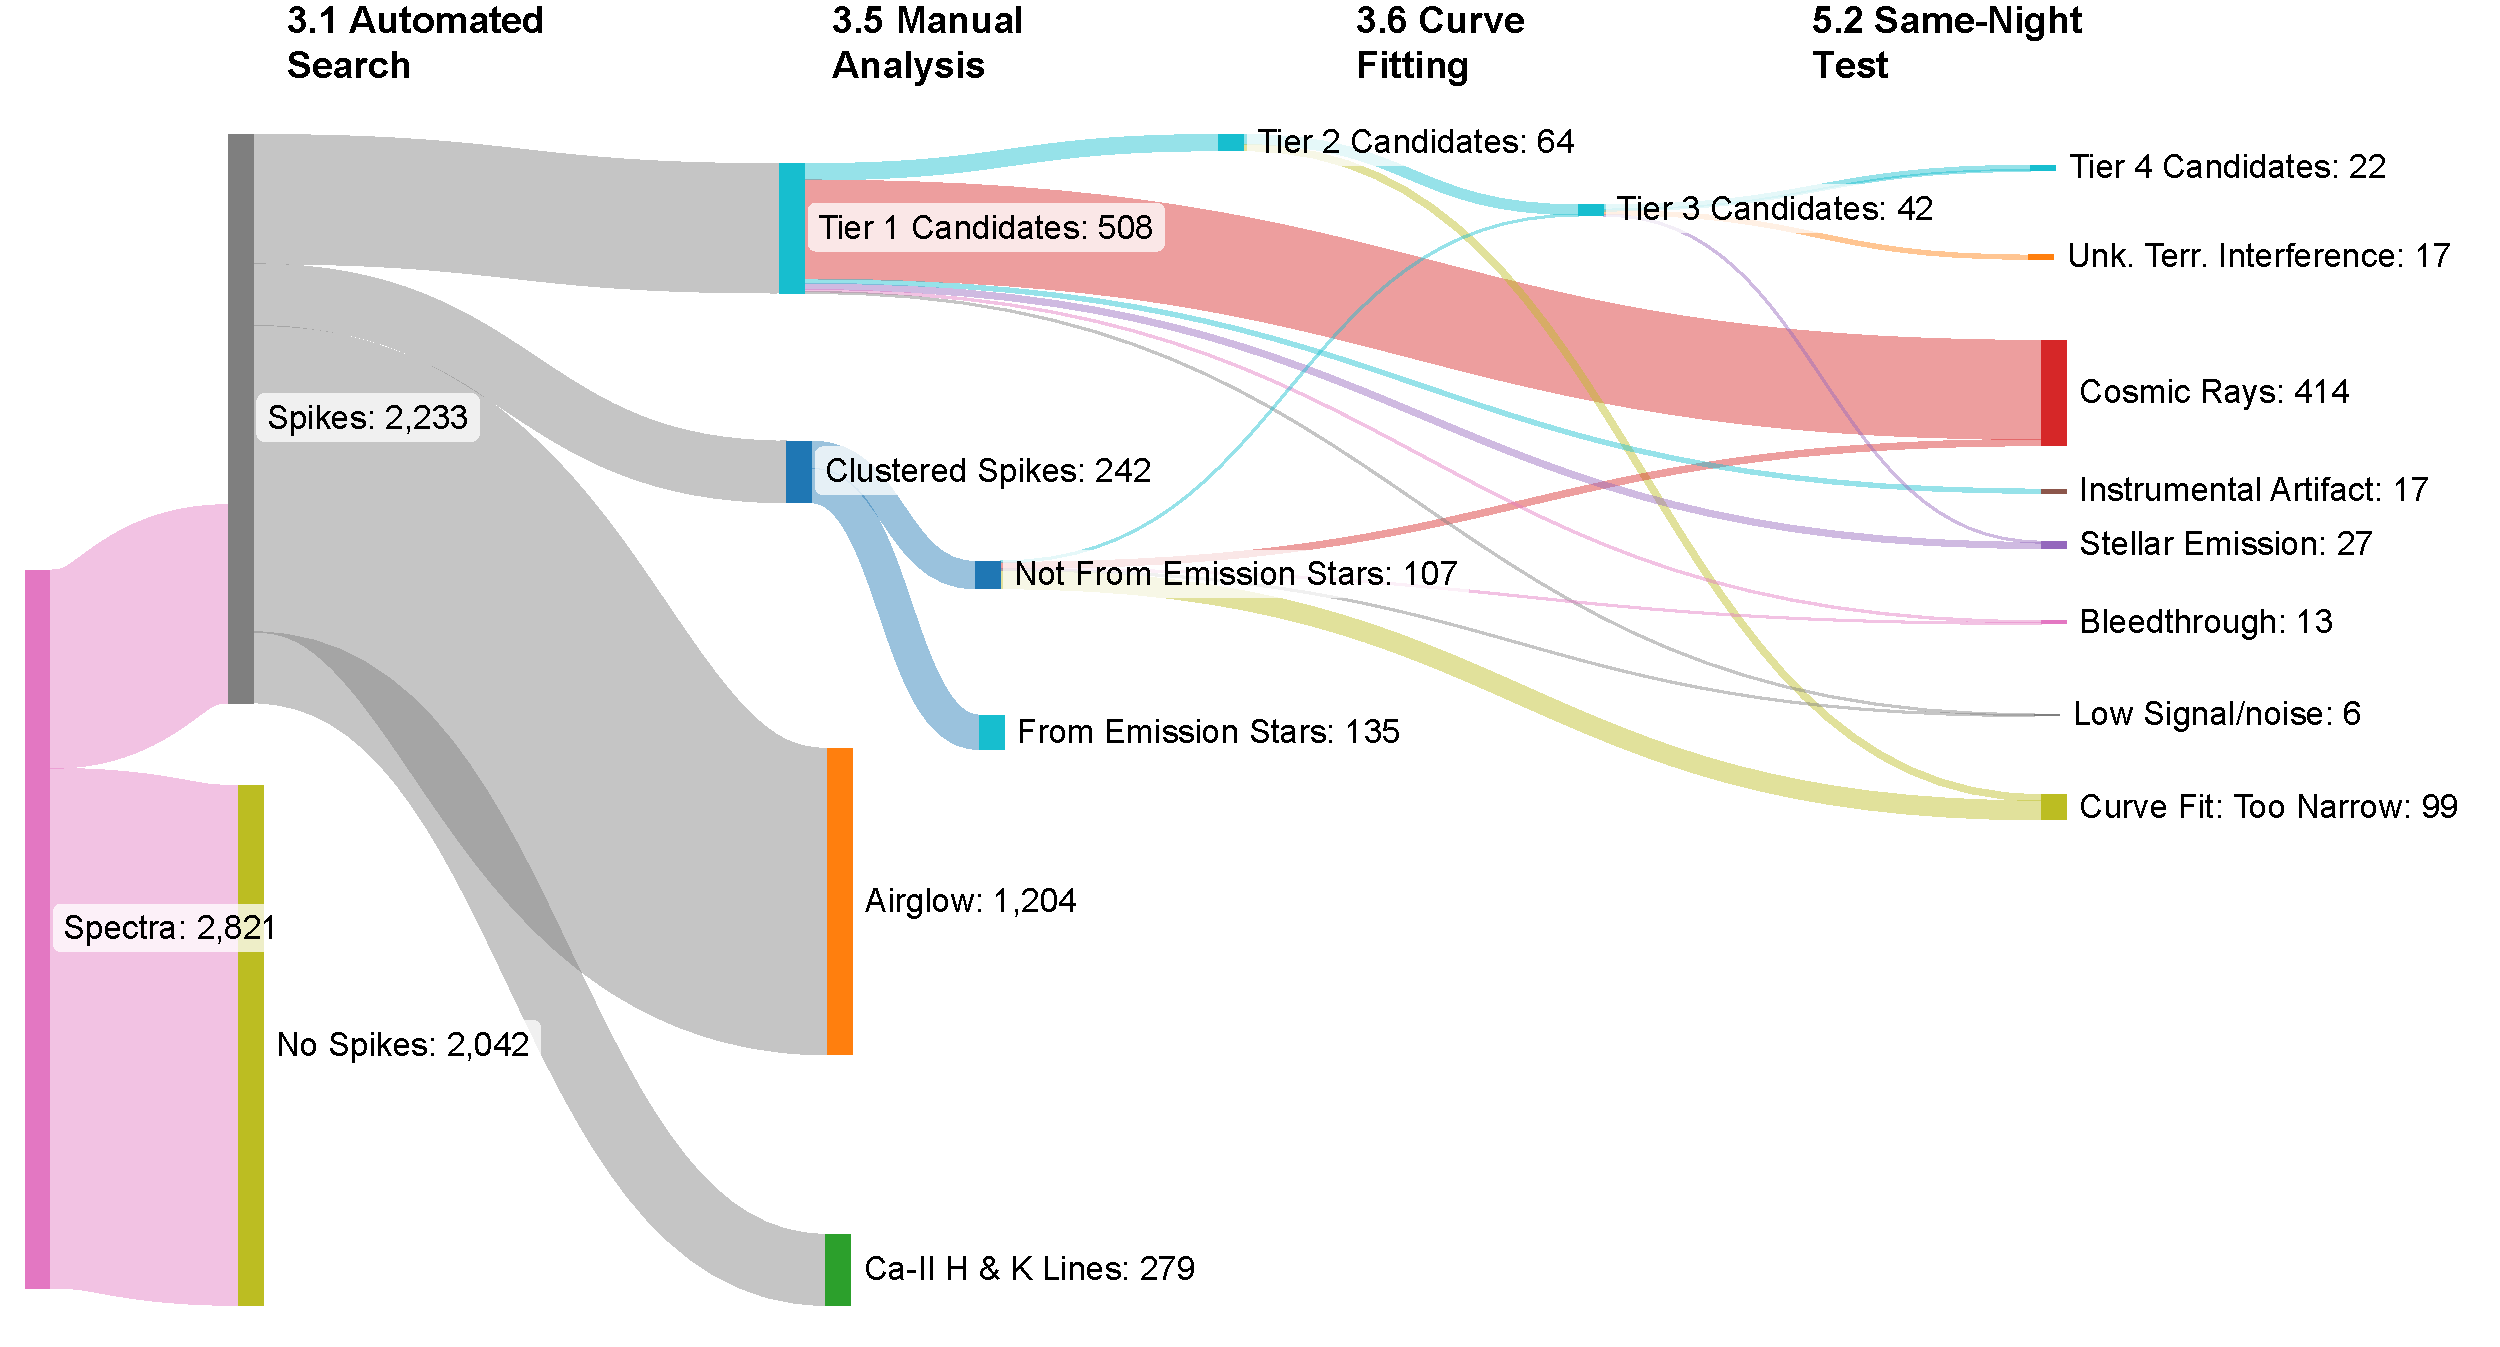
\includegraphics[width=\textwidth]{sankey.pdf}
    \caption{The number of candidates identified or eliminated in each stage of our search process. Line thicknesses are proportional to number of candidates of that type.  The pink bands indicate number of spectral files analyzed; thereafter, the numbers represent number of candidate spikes, possibly more than one per file.  See text for details and discussion.}
    \label{fig:sankey}
\end{figure*}

Figure \ref{fig:sankey} summarizes our search flow, and provides the number of spikes that fall into each category at each phase of the search.  Our automated search algorithm identified 508 Tier 1 candidates, plus 242 spikes that appeared in clusters of more than four per star.  107 of these were not from known emission-type stars, and were manually inspected along with the other Tier 1 candidates.  This led to 64 Tier 2 candidates, whose line widths were estimated as per Section \ref{s:curvefit}: 42 of them met the criterion of Eq. \ref{eq:linewidth} and became Tier 3 candidates.

\section{Further Analysis of Tier 3 Candidates}

Having reduced the dataset to 42 promising candidates, we subjected them to detailed scrutiny to identify sources of possible terrestrial contamination.

\subsection{Detailed Inspection of the  \DIFaddbegin \DIFadd{HD 127423 }\DIFaddend Candidate} 
 \DIFaddbegin \label{s:HD 127423}
\DIFaddend 

One Tier 3 candidate, a spike at 5732.945~\AA\DIFaddbegin \DIFadd{~}\DIFaddend in an observation of  \DIFaddbegin \DIFadd{HD 127423 }\DIFaddend dated 2014-10-06 10:06:38.740, seemed especially intriguing.  \DIFaddbegin \DIFadd{HD 127423 }\DIFaddend is a G-Type star  \DIFaddbegin \DIFadd{and the candidate did not match Calcium H and K wavelengths. The }\DIFaddend peak was not near \DIFaddbegin \DIFadd{any }\DIFaddend terrestrial airglow lines \DIFaddbegin \DIFadd{. It }\DIFaddend had a gaussian lineshape close to the instrument's FWHM \DIFaddbegin \DIFadd{. As }\DIFaddend seen in Figure  \DIFaddbegin \DIFadd{\ref{fig:seti_candidate_HD 127423}, the candidate's }\DIFaddend spectral energy is entirely within the CCD image of the spectrometer's entry slit,  \DIFaddbegin \DIFadd{which implies }\DIFaddend that this is not a cosmic ray or calibration lamp bleed-through. We subjected it to additional detailed analysis.

\begin{figure*}
    \centering
      \DIFaddbeginFL \begin{overpic}[width=.8\textwidth]{seti_candidate_HD127423.pdf}
     \put(75,40){\textcolor{red}{Star: HD 127423}}  %DIF >  adjust (x,y) % coordinates
    \end{overpic}
    \DIFaddendFL \caption{Star:  \DIFaddbeginFL \DIFaddFL{HD 127423}\DIFaddendFL , Spectral Type:G0V, Observation Date/Time: 2013-06-01, 04:16:19.375. Top panel: reduced spectrum.  Bottom panel: subsection of the corresponding CCD image for this wavelength range. \DIFaddbeginFL \DIFaddFL{Wavelengths in both the reduced 1-D spectrum and the 2-D CCD image are shown in the terrrestrial (observatory) reference frame.}\DIFaddendFL }
     \DIFaddbeginFL \label{fig:seti_candidate_HD 127423}
\DIFaddendFL \end{figure*}

The calibration lamp was on during the observation, and bleedthrough is observed at some wavelengths, but not at the candidate wavelength of 5732.93~\AA.

This candidate does not meet our criteria for natural stellar emission lines (Section \ref{s:stellaremission}).  The line occurs in isolation, and its linewidth is exceptionally narrow (just above the instrument's  \DIFaddbegin \DIFadd{LSF). HD 127423 }\DIFaddend is of spectral type G0V, which do not generally have emission spectra besides \DIFaddbegin \DIFadd{Calcium }\DIFaddend H and K lines \citep{HandKemissionlines}, which do not match the candidate's wavelength. 

The candidate does not match any known airglow lines listed in the UVES database \citep{faint_airglow_database} \citep{UVES_database}. 

We considered the possibility of human laser interference by overflying LiDAR satellites and drones.  A review of LiDAR technologies found that our candidate at 5733~\AA~does not match the wavelengths used by LiDAR satellites (5320~\AA, 3550~\AA, and 10640~\AA\DIFaddbegin \DIFadd{~}\DIFaddend \citep{lidar_history}), airborne LiDAR systems (10640~\AA, \citep{lidar_history}), autonomous vehicles (9050~\AA\DIFaddbegin \DIFadd{~}\DIFaddend and 15500~\AA\DIFaddbegin \DIFadd{~}\DIFaddend \citep{vehicle_lidar}), and oceanic bathymetric LiDAR systems (5320~\AA, \citep{bathymetric_lidar}). 

We also considered interference from ground-based adaptive optics lasers. However, ESO's adaptive optics lasers excite atmospheric sodium lines at 5890~\AA, which does not match our candidate and which would have been filtered out as an airglow line \citep{HARPS_guidestars}. In general, Laser Guidestar Adaptive Optics (LGAO) systems work by artificially inducing airglow \citep{LaserGuideStarAdaptiveOptics}, and would be ignored by our airglow rejection filter.  Other adaptive optics systems can utilize Raleigh scattering instead of artificially induced airglow--but these systems generally operate at blue wavelengths \citep{RaleighScattering} rather than the yellow/green range of the  \DIFaddbegin \DIFadd{HD 127423 }\DIFaddend candidate.

The  \DIFaddbegin \DIFadd{HD 127423 }\DIFaddend candidate is not a frequently observed feature that might represent an instrumental artifact, spurious byproduct of the blaze function or reduction pipeline error.  Our analysis in Section \ref{s:repeat} shows that this spike does not recur in other observations of this star.  Analysis by Nikolai Piskunov (pers. comm.) noted that no recurring spike at this wavelength was observed in a random sample of 396 HARPS spectra. 

However, there is also overwhelming evidence that this signature could not have arrived from interstellar distances.  

The spike in question only appears once in all 8 observations of  \DIFaddbegin \DIFadd{HD 127423 }\DIFaddend available in the HARPS database. However, as noted by N. Piskunov (pers. comm.), it appears in observations of \emph{other} stars taken on the same night, including  \DIFaddbegin \DIFadd{HD 107181, HD 128356, HD 126535, HD 143120, HD 143361, HD 144899.  }\DIFaddend Each of these observations showed a spike at or near 5733\DIFaddbegin \DIFadd{~}\DIFaddend \AA, even though the stars were separated by hours of right ascension. The eight observations were taken within a two-hour window, with a 15-minute exposure time for each consecutive observation. The odds that extraterrestrials beaming lasers from stars at such varied distances would all happen to have their signals arriving at Earth at the same time seemed small. 

We can deduce whether these spikes originate from the stars in question, or from a terrestrial source, by considering their Doppler shifts.  When we Doppler-shifted the spectra from the standardized barycentric reference frame into each star's respective stellar reference frame (Figure \ref{fig:stellarframespectra}), we observed that absorption features common to all these stars align, but the spike does not. Thus, the signal is not in the stars' reference frames.  When we Doppler-shifted each spectrum into the {\em terrestrial} observatory's reference frame using the barycentric radial velocity listed in the using the \texttt{HIERARCH ESO DRS BERV} FITS header, we find that the stars' absorption features do not line up, but the mysterious spike does.

 \DIFaddbegin \begin{figure}
    \DIFaddendFL \centering
    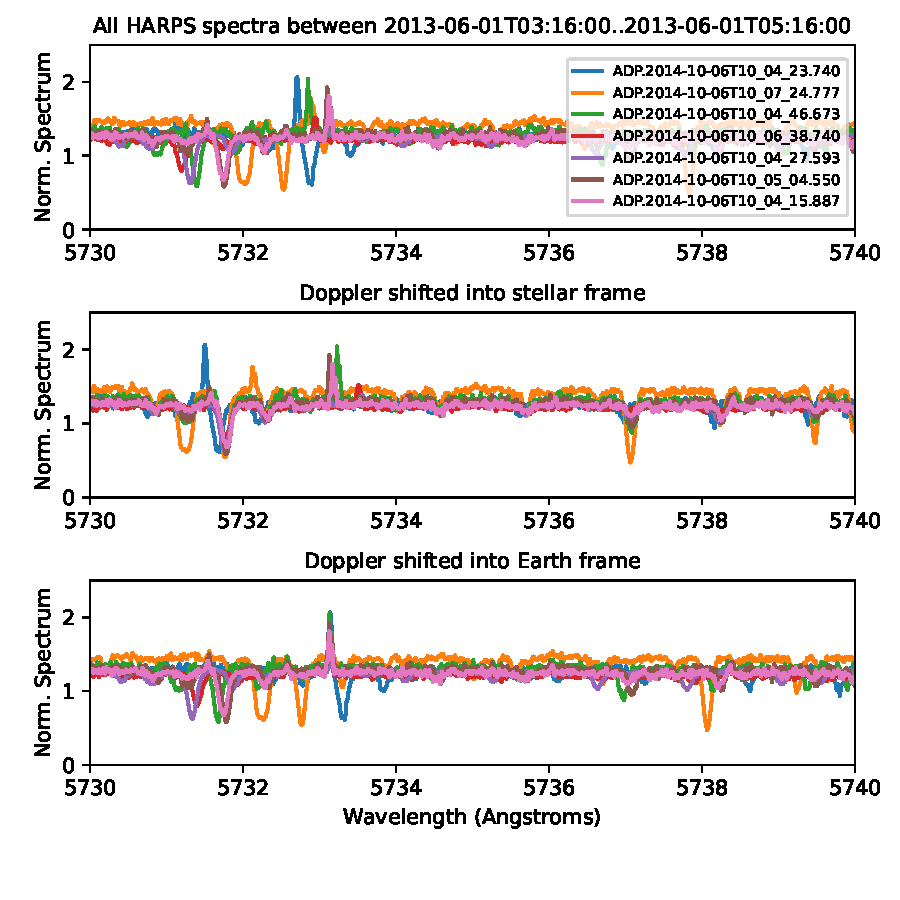
\includegraphics[width=\columnwidth]{stellarframespectra.pdf}
    \caption{Reduced spectra for all stars observed by HARPS within +/- 1 hour of the  \DIFaddbeginFL \DIFaddFL{HD 127423 }\DIFaddendFL candidate at 2013-06-01, 04:16:19.375 ( \DIFaddbeginFL \DIFaddFL{HD 127423}\DIFaddendFL ,  \DIFaddbeginFL \DIFaddFL{HD 107181}\DIFaddendFL ,  \DIFaddbeginFL \DIFaddFL{HD 128356}\DIFaddendFL ,  \DIFaddbeginFL \DIFaddFL{HD 126535}\DIFaddendFL ,  \DIFaddbeginFL \DIFaddFL{HD 143120}\DIFaddendFL ,  \DIFaddbeginFL \DIFaddFL{HD 143361 }\DIFaddendFL and  \DIFaddbeginFL \DIFaddFL{HD 144899}\DIFaddendFL ).  Each observation shows a spike around 5733~\AA. Top panel: all 7 spectra in the default reference frame for HARPS pipeline (solar system barycenter). Middle panel: all 7 spectra, doppler shifted to the reference frame of each respective star. Bottom panel: all 7 spectra, Doppler shifted into the Earth's reference frame.  The alignment of the 5733{\DIFaddbeginFL \DIFaddFL{~}\DIFaddendFL \AA} spikes in the terrestrial reference frame indicates that this is a terrestrial signal, not a stellar feature.}
    \label{fig:stellarframespectra}
 \DIFaddbeginFL \end{figure}
\DIFaddend 

 We confirmed that the spike was in the observatory's reference frame by looking at the raw CCD images, which showed a common spike at the same CCD pixels in all of them.  There was no evidence of CCD  \DIFaddbegin \enquote{bleed-through} \DIFaddend at this location, and these features appear at the same pixel position on the CCD images, confirming that there is no doppler shift at all relative to the calibration source. Thus, our analysis suggests that this is an as yet unknown terrestrial source.

The two-hour time window during which the source persisted argues against satellites in low earth orbit, since at such velocities the satellite would not stay in the same location long enough to continuously beam down a laser for that duration. However, we can also rule out a transmitter at interstellar distances. We were therefore left with a signature which is unexplained, yet originating from a local source. 

\subsection{Tier 4:  \DIFaddbegin \DIFadd{Same Night }\DIFaddend Doppler Detection of Unknown Terrestrial Sources}
\label{s:doppler}
Having identified an unknown terrestrial source for  \DIFaddbegin \DIFadd{HD 127423 (Section \ref{s:HD 127423}}\DIFaddend ) by looking for the same spike in contemporaneous observations in the terrestrial reference frame,  we repeated this process for the other Tier 3 candidates (Figure \ref{fig:sankey}). Of our 35 Tier 3 candidates, 13 showed up in observations of other stars within a four-hour window on the same night, and appear stationary in the terrestrial reference frame. They are listed in \DIFaddbegin \DIFadd{Table }\DIFaddend \ref{table:terrestrial_interference}. A couple of these mystery terrestrial sources recur multiple times (particularly around 5733~\AA~and 5826 \DIFaddbegin \DIFadd{~}\DIFaddend \AA), while others show up only once and are distributed throughout HARPS' wavelength range. Although no longer viable SETI candidates, these terrestrial anomalies may be of meteorological interest. In future work we will subject them to closer scrutiny, which we hope will allow a more robust optical SETI search.

We also recategorized a few of our candidates as stellar emission lines at this stage.  Thus, we were left with 22 candidate spikes which may represent unknown extraterrestrial sources.  These are listed in Table \ref{t:corecandidates}.

\begin{table}
\centering
\begin{tabular}{|l|l|l|c|}
\hline
     & Spectral & Wavel. & \\
Star &  Type & (\DIFaddbeginFL \DIFaddFL{~}\DIFaddendFL \AA) & Observation Time \\
\hline
 \DIFaddbeginFL \DIFaddFL{GJ 3827   }\DIFaddendFL & K1V   & 5946.32 & 2005-05-05 04:16:30.575\\
 \DIFaddbeginFL \DIFaddFL{HD 127423 }\DIFaddendFL & G0V   & 5732.95 & 2013-06-01 04:16:19.375\\
 \DIFaddbeginFL \DIFaddFL{HD 127423 }\DIFaddendFL & G0V   & 5826.18 & 2013-06-01 04:16:19.375\\
 \DIFaddbeginFL \DIFaddFL{HD 127423 }\DIFaddendFL & G0V   & 5998.05 & 2013-06-01 04:16:19.375\\
 \DIFaddbeginFL \DIFaddFL{HD 165204 }\DIFaddendFL & G6/8V & 5826.58 & 2013-06-01 07:25:43.745\\
 \DIFaddbeginFL \DIFaddFL{HD 21759  }\DIFaddendFL & G8/K1 & 5773.35 & 2012-12-28 03:16:30.165\\
 \DIFaddbeginFL \DIFaddFL{HD 34642  }\DIFaddendFL & G3V   & 4358.13 & 2018-02-01 01:42:30.839\\
 \DIFaddbeginFL \DIFaddFL{HD 34642  }\DIFaddendFL & G3V   & 5460.50 & 2018-02-01 01:42:30.839\\
 \DIFaddbeginFL \DIFaddFL{HD 94126  }\DIFaddendFL & G8IV  & 5453.17 & 2013-06-01 01:19:53.391\\
 \DIFaddbeginFL \DIFaddFL{HD 94126  }\DIFaddendFL & G8IV  & 5825.85 & 2013-06-01 01:19:53.391\\
 \DIFaddbeginFL \DIFaddFL{HD 94126  }\DIFaddendFL & G8IV  & 5945.87 & 2013-06-01 01:19:53.391\\
 \DIFaddbeginFL \DIFaddFL{HIP 59341 }\DIFaddendFL & G5V   & 5732.82 & 2013-06-01 03:04:25.906\\
 \DIFaddbeginFL \DIFaddFL{HIP 59341 }\DIFaddendFL & G5V   & 5826.05 & 2013-06-01 03:04:25.906\\
\hline
\end{tabular}
\caption{Candidates identified as unknown terrestrial sources, which appear in multiple separate stars observed on the same night, and are stationary in the telescope's reference frame.}
\label{table:terrestrial_interference}
\end{table}

\begin{table*}
\centering
\begin{tabular}{|l|l|l|c|}
\hline
     & Spectral& Wavel.& \\
Star & Type & (\DIFaddbeginFL \DIFaddFL{~}\DIFaddendFL \AA) & Obs date/time \\
\hline
BD-114672 & K7V & 6477.500 & 2023-06-03 09:09:16.351 \\
CD-4911401 & N/A & 5823.985 & 2005-05-31 03:51:05.988 \\
 \DIFaddbeginFL \DIFaddFL{CoRot-24 }\DIFaddendFL & K1V & 5983.375 & 2012-11-20 05:56:02.541 \\
 \DIFaddbeginFL \DIFaddFL{CoRot-32 }\DIFaddendFL & K0V & 6173.490 & 2012-01-27 02:14:50.135 \\
 \DIFaddbeginFL \DIFaddFL{CoRot 101614469 }\DIFaddendFL &  & 5593.895 & 2008-07-25 04:50:31.896 \\
 \DIFaddbeginFL \DIFaddFL{CoRot 221699621 }\DIFaddendFL & K0V & 5446.725 & 2011-12-03 06:43:16.408 \\
 \DIFaddbeginFL \DIFaddFL{GJ 1214 }\DIFaddendFL & M4.5V & 4784.190 & 2012-07-10 00:39:39.961 \\
 \DIFaddbeginFL \DIFaddFL{GJ 1236 }\DIFaddendFL & M4V & 5975.520 & 2012-05-15 07:27:46.968 \\
 \DIFaddbeginFL \DIFaddFL{GJ 3053 }\DIFaddendFL & M4.5 & 3854.260 & 2016-01-23 01:11:31.273 \\
 \DIFaddbeginFL \DIFaddFL{GJ 317 }\DIFaddendFL & M3.5V & 4662.790 & 2018-04-10 03:25:08.275 \\
 \DIFaddbeginFL \DIFaddFL{GJ 3221 }\DIFaddendFL & M3.5V & 6688.415 & 2011-09-25 07:25:30.812 \\
 \DIFaddbeginFL \DIFaddFL{GJ 3535 }\DIFaddendFL & G3V & 6769.710 & 2004-05-31 00:36:26.077 \\
 \DIFaddbeginFL \DIFaddFL{HD 110411 }\DIFaddendFL & A0Va\_lB & 5709.510 & 2006-02-10 07:02:59.081 \\
 \DIFaddbeginFL \DIFaddFL{HD 147644 }\DIFaddendFL & F8V & 5937.510 & 2015-04-19 06:48:21.114 \\
 \DIFaddbeginFL \DIFaddFL{HD 184711 }\DIFaddendFL & G5wA/F & 6566.015 & 2008-09-20 00:41:44.834 \\
 \DIFaddbeginFL \DIFaddFL{HD 197623 }\DIFaddendFL & G3V & 6351.400 & 2005-05-18 09:10:45.139 \\
 \DIFaddbeginFL \DIFaddFL{HD 223171 }\DIFaddendFL & G2V & 6769.420 & 2015-12-16 01:26:43.087 \\
 \DIFaddbeginFL \DIFaddFL{HD 34642 }\DIFaddendFL & G3V & 5769.340 & 2018-02-01 01:42:30.839 \\
 \DIFaddbeginFL \DIFaddFL{HD 59088 }\DIFaddendFL & O6f & 4365.010 & 2006-03-26 00:02:33.378 \\
 \DIFaddbeginFL \DIFaddFL{HIP 87607 }\DIFaddendFL & M0V & 4632.245 & 2012-10-22 23:39:09.238 \\
WASP-19 & G8V & 6054.870 & 2020-02-15 04:09:40.886 \\
WASP-89 & K3 & 5198.055 & 2012-10-03 05:01:01.142 \\
\hline
\end{tabular}
\caption{Tier 4 candidates which pass all our selection criteria.}
\label{t:corecandidates}
\end{table*}

Spectral and CCD images of three of these Tier 4 candidates are shown in Figures \ref{fig:seti_candidate_CD-312415},  \DIFaddbegin \DIFadd{\ref{fig:seti_candidate_HIP 87607}, and \ref{fig:seti_candidate_GJ 317}}\DIFaddend .

\begin{figure*}
    \centering
      \DIFaddbeginFL \begin{overpic}[width=.8\textwidth]{HD34642Version3pdf.pdf}
     \put(70,60){\textcolor{red}{Star: HD 34642}}  %DIF >  adjust (x,y) % coordinates
    \end{overpic}
    \DIFaddendFL \caption{Star:  \DIFaddbeginFL \DIFaddFL{HD 34642}\DIFaddendFL , Spectral Type: K0IV, Observation Date/Time: 2018-02-01, 01:42:30.839. Top panel: reduced spectrum. Bottom panel: subsection of the corresponding CCD image for this wavelength range. \DIFaddbeginFL \DIFaddFL{Wavelengths in both the reduced 1-D spectrum and the 2-D CCD image are shown in the terrestrial (observatory) reference frame.}\DIFaddendFL }
    \label{fig:seti_candidate_CD-312415}
\end{figure*}

%DIF > \begin{figure*}
    %DIF > \centering  
  %DIF >   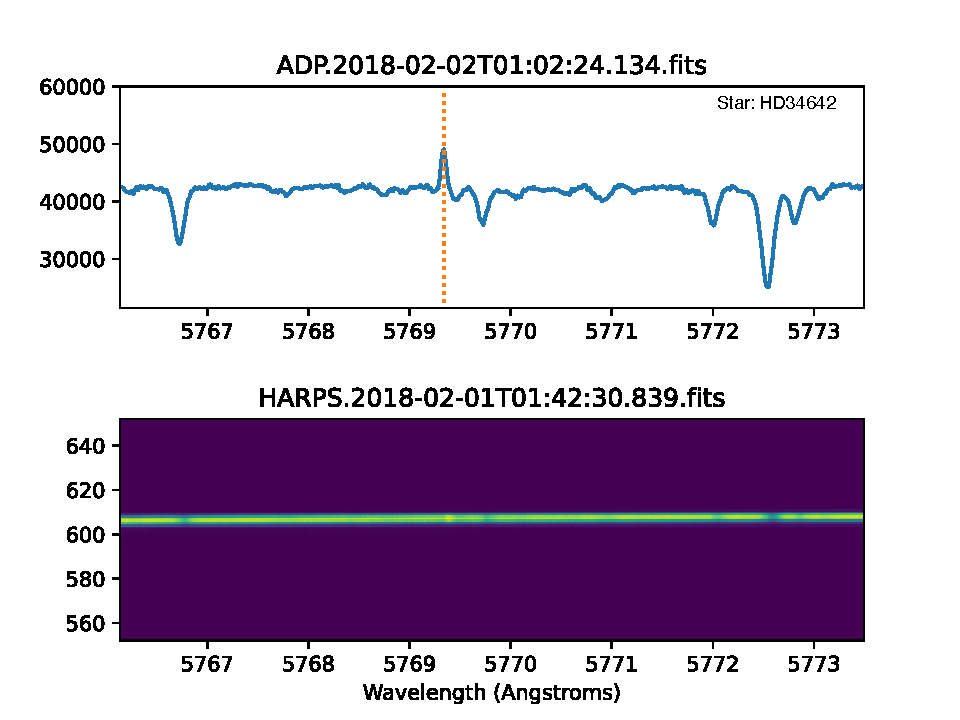
\includegraphics[width=.8\textwidth]{HD34642Version3pdf.pdf}
   %DIF >  \caption{Star: HD 34642, Spectral Type: K0IV, Observation Date/Time: 2018-02-01, 01:42:30.839.  Top panel: reduced spectrum.  Bottom panel: subsection of the corresponding CCD image for this wavelength range. Wavelengths in both the reduced 1-D spectrum and the 2-D CCD image are shown in the terrrestrial (observatory) reference frame.}
  %DIF >   \label{fig:seti_candidate_CD-312415}
%DIF > \end{figure*}
\DIFaddbegin 

\DIFaddend \begin{figure*}
    \centering
      \DIFaddbeginFL \begin{overpic}[width=.8\textwidth]{HIP87607figureforpaper2.pdf}
     \put(70,60){\textcolor{red}{Star: HIP 87607}}  %DIF >  adjust (x,y) % coordinates
    \end{overpic}
     \DIFaddendFL \caption{Star:  \DIFaddbeginFL \DIFaddFL{HIP 87607}\DIFaddendFL , Spectral Type: M0V, (Observation Date/Time: 2012-10-22, 23:39:09.238) Top panel: reduced spectrum. Bottom panel: subsection of the corresponding CCD image for this wavelength range.}
     \DIFaddbeginFL \label{fig:seti_candidate_HIP 87607}
\DIFaddendFL \end{figure*}

\begin{figure*}
    \centering
     \DIFaddbeginFL \begin{overpic}[width=.8\textwidth]{seti_candidate_GJ317.pdf}
     \put(80,37){\textcolor{red}{Star: GJ 317}}
    \end{overpic}
    \DIFaddendFL \caption{Star:  \DIFaddbeginFL \DIFaddFL{GJ 317}\DIFaddendFL , Spectral Type: M3.5V, (Observation Date/Time: 2018-04-10, 03:25:08.275) Top panel: reduced spectrum. Bottom panel: subsection of the corresponding CCD image for this wavelength range.}
     \DIFaddbeginFL \label{fig:seti_candidate_GJ 317}
\DIFaddendFL \end{figure*}

\section{Searching for Repeat Occurrences}
\label{s:repeat}
While laser transmissions could be ephemeral, signals that recur consistently would arguably be stronger candidates since they provide reproducible evidence and are less likely to be random noise or cosmic ray hits.  Therefore, we repeated our analysis for {\em all} available observations of each of the 22 stars which yielded at least one Tier 4 candidate signal. In this search, we performed the curve fitting analysis (Section \ref{s:curvefit}) before manual analysis (Section \ref{s:falsepositive}) to reduce the manual labor required.  

Of 696 additional observations of these 17 stars, our automated search algorithm (Section \ref{s:automated}) and curve fitting algorithm (Section \ref{s:curvefit}) yielded a total of 442 candidates that satisfied the curve fitting criteria (including the original candidates from Section \ref{s:results}).  We repeated our analyses from Sections \ref{s:falsepositive}, and \ref{s:doppler} on these observations, and categorized 335 as cosmic rays, 19 as instrumental artifacts, 6 calibration lamp bleedthrough, 7 with signal/noise ratio too low to assess, and 9 as terrestrial interference based on the  \DIFaddbegin \enquote{same-night test} \DIFaddend (Section \ref{s:doppler}). This left a total of 66 candidates for further analysis, including the 22 found by the original search.  This search is summarized in Figure \ref{fig:sankey_repeater} and the new candidates identified in this stage are listed in Appendix \ref{s:repeat_candidates}.

\begin{figure}
    \centering
    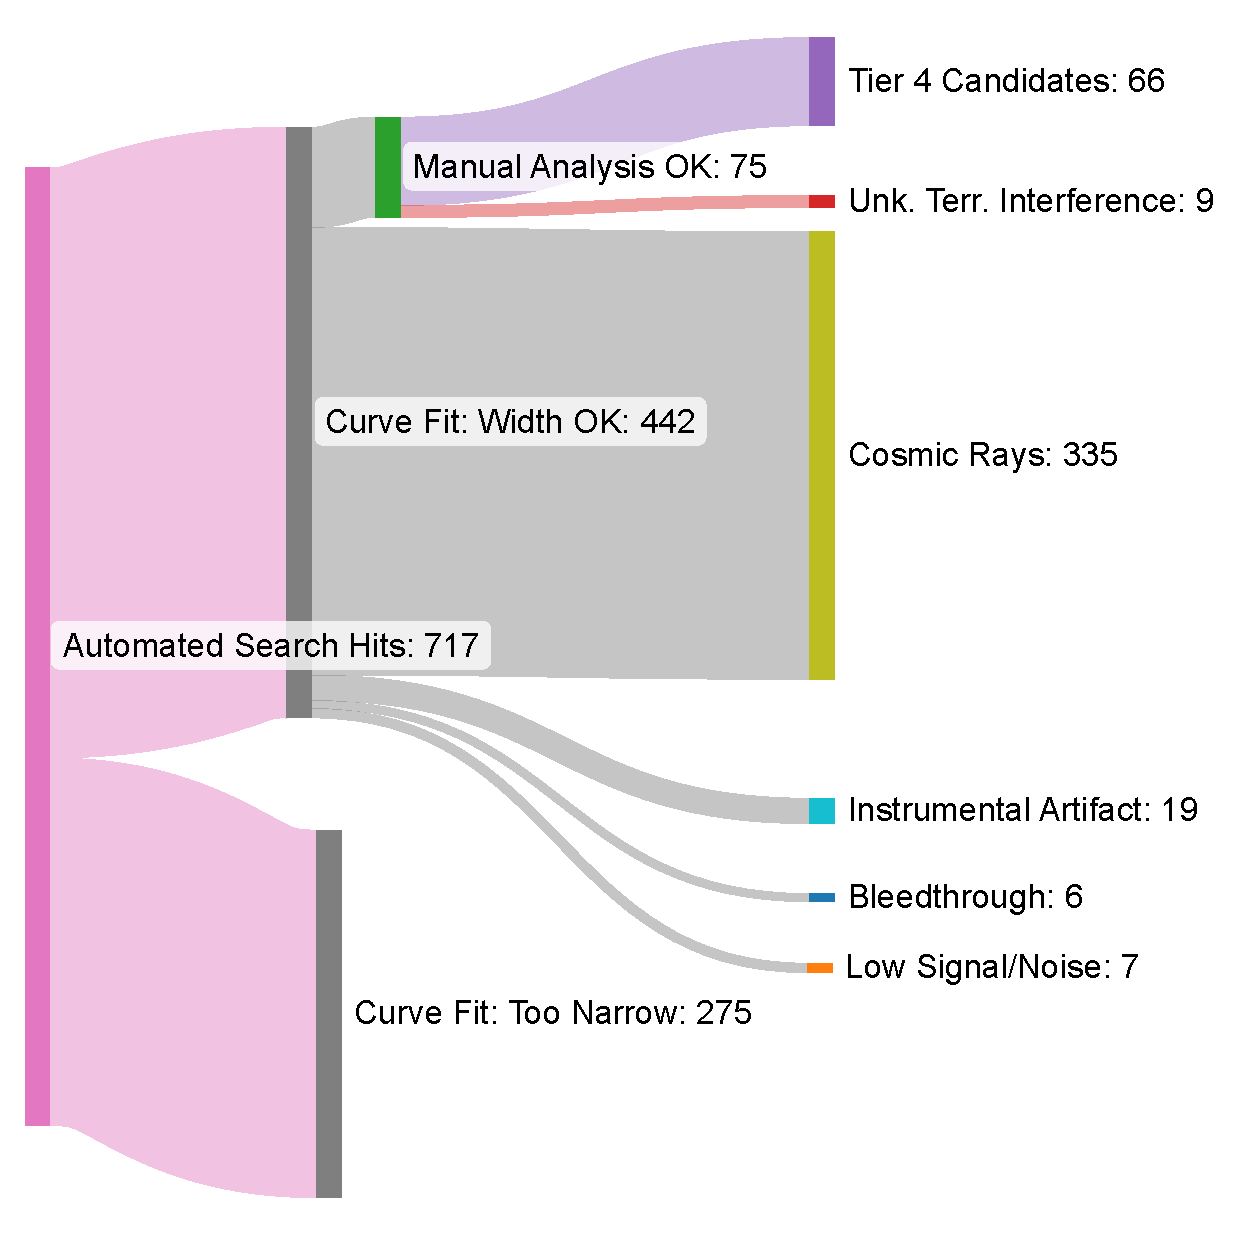
\includegraphics[width=\columnwidth]{sankey_repeater.pdf}
    \caption{The number of candidates identified or eliminated in each stage of our search for repeat occurrences of spikes in other observations of the core candidates from Table \ref{t:corecandidates}.  
    Line thicknesses are proportional to number of candidates of that type.  This diagram includes the 22 identified previously in Section \ref{s:results}, Table \ref{t:corecandidates} and Figure \ref{fig:sankey}.  See text for details and discussion.}
    \label{fig:sankey_repeater}
\end{figure}

\begin{figure}
    \centering
    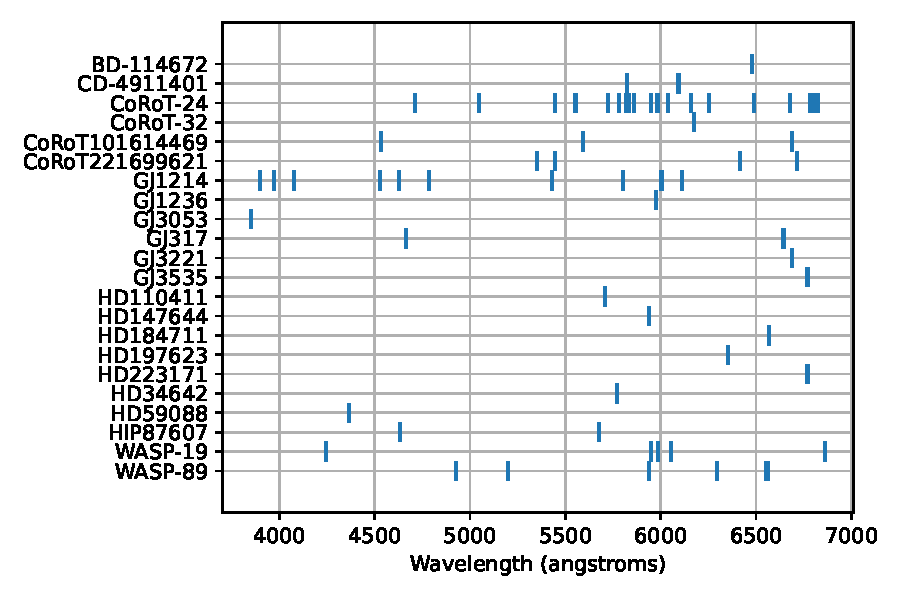
\includegraphics[width=\columnwidth]{candidate_wavelengths.pdf}
    \caption{Distribution of wavelengths of Tier 4 candidate spikes identified in all observations of each candidate star.}
    \label{fig:candidate_wavelengths}
\end{figure}

While some stars had candidate spikes in several different observations, they were almost always at very different wavelengths, hundreds of angstroms apart (Figure \ref{fig:candidate_wavelengths}).  The closest pair of spikes (separated by .07~\AA) is not a recurring feature, but a  \DIFaddbegin \DIFadd{closely spaced  double spike from }\DIFaddend the same observation \DIFaddbegin \DIFadd{time}\DIFaddend . The second-closest is in  \DIFaddbegin \DIFadd{CoRot-24}\DIFaddend : two observations of  \DIFaddbegin \DIFadd{CoRot-24 }\DIFaddend at 5552.13\DIFaddbegin \DIFadd{~\AA~}\DIFaddend and 5553.72~\AA~on 2011-12-04 at 05:29:17.513 and 01:46:11.545 respectively.  These are separated by 1.6~\AA.  If these were the same source observed at two different Doppler shifts, the relative velocity of source and receiver would need to change by 44 km/s in 4 hours. Whether this is the same source or just coincidence will be the subject of future work. Several  other stars (CD-4911401,  \DIFaddbegin \DIFadd{GJ 317}\DIFaddend , WASP-19,  \DIFaddbegin \DIFadd{GJ 1214, HIP 87607, CoRot  101614469, CoRot  22169962}\DIFaddend ) showed additional candidates in subsequent observations--but none which repeated at the same wavelength as the initial detection. 

\section{Summary and Conclusions}
We analyzed single archived reduced spectra from 2821 stellar targets taken by the ESO’s HARPS spectroscope to search for potential signatures of lasers from extraterrestrial civilizations. We identified false positives (Section \ref{s:falsepositive}), including cosmic rays (Section \ref{s:cosmic}), bleed through from the Th-Ar calibration lamp (Section \ref{s:bleedthrough}), night sky airglow lines (Section \ref{s:Airglow}), and large clusters of emission lines which are likely the product of natural stellar activity (Section \ref{s:stellaremission}). Of the 2821 stellar spectra we analyzed, we identified 508 Tier 1 candidates with at least one narrow spectral emission feature.  64 of these did not fit any of the above false positive categories, becoming Tier 2 candidates. We filtered this dataset further on the basis of linewidth (Section \ref{s:curvefit}). We were left with a total of 42 compelling Tier 3 candidates (Section \ref{s:results}). We then looked for terrestrial interference by comparing each candidate to observations of other stars taken within a four hour window, looking for matching spikes in the terrestrial reference frame.  This eliminated 17 candidates as likely terrestrial interference (Section \ref{s:doppler}). Although the 17 spikes we eliminated are definitely terrestrial in origin, their cause is unknown.  The multi hour window during which they appeared argues against a laser from a classified satellite in Low Earth Orbit. They also might represent novel atmospheric phenomena and could be of interest to meteorologists. This left 22 Tier 4 candidates which passed through all of our filters for prosaic explanations and currently show no indication of being terrestrial in origin, and therefore warrant further investigation as SETI candidates. To search for any repeat occurrences of candidate signals, we searched the available additional observations of any star that yielded a Tier 4 candidate, totaling 696 additional spectra. These  \DIFaddbegin \enquote{repeater} \DIFaddend candidates were subjected to all of the same false positive filters as our initial candidates, yielding an additional 44 candidates for a total of 66. One observation of M-dwarf star  \DIFaddbegin \DIFadd{CoRot-24 }\DIFaddend yielded two spikes in separate observations only 1.6~\AA~apart in wavelength. Whether this is an example of a repeating signal or just coincidence will be the subject of additional followup analysis. All of the other additional unexplained spikes uncovered in the search for repeat occurences showed up at very different wavelengths. However, regardless of their transient and non-repeating nature, all of our final candidates survived a battery of tests which eliminated many natural and anthropogenic false positives. Therefore, they warrant further investigation.

The 22 stars that yielded candidates run a wide gamut of spectral types, each of which have different implications for possible astrophysical explanations. Many G and K type stars do not have many emission lines, aside from  Calcium H and K lines, which we automatically filtered out. M type stars represent a more nuanced case. Detection of candidate laser signals is more ambiguous in red dwarfs due to their relatively cool temperatures, high metallicity, and chromosopheric/magnetic activity, which leads to flaring and prominent narrow emission lines\DIFaddbegin \DIFadd{, as noted by }\DIFaddend \citep{Marcy_2021}. As we discuss in Section \ref{s:future}, developing more robust tools to differentiate M-dwarf stellar activity from possible laser emissions will be a priority in our future investigations. 

A goal of this study was to build pipelines and identify obstacles to future, more comprehensive searches (See Section \ref{s:future}).  One challenge we identified is the difficulty of categorizing cosmic ray hits.  While visual inspection can easily spot cosmic ray hits that form linear tracks, it can be  \DIFaddbegin \DIFadd{difficult  }\DIFaddend to visually distinguish direct cosmic ray hits onto the region of the CCD illuminated by starlight from real spectral lines.  Thus, some  of our candidates  \DIFaddbegin \DIFadd{may still }\DIFaddend be cosmic ray hits.  Automated detection of cosmic ray false positives is a priority for the future which we will discuss in Section \ref{s:automatic_cosmic_ray}. 

Since our study analyzed only one observation from each target and then performed follow-up analysis of additional observations only on stars where a candidate was found, it can only constrain the likelihood of continuous sources repeatedly directed toward Earth. It could easily miss more intermittent signals. Thus, our study must contend with the longstanding challenge faced by many other SETI searches: how can we adapt our methodologies to account for the possibility of intermittent transmitters or  \DIFaddbegin \enquote{one-off} \DIFaddend signals?  Can  \DIFaddbegin \enquote{one-off} \DIFaddend signals constitute SETI detections, or is repeatability an inescapable requirement of a confirmed detection \citep{2019nasatechnosignatures, Wow!Signal}? These questions will define the future direction of this project.

\section{Future Avenues of Research}
\label{s:future}

\subsection{Expanding the Search}
Our search only analyzed one observation from each star. While we did look at all other observations of the handful of stars which yielded compelling candidates, our search technique is not yet automated enough to survey a larger dataset.  The present work analyzed about 3400 observations, which required manual visual inspection of about 1000 Tier 1 candidates (Fig. \ref{fig:sankey} and \ref{fig:sankey_repeater}).

In future work, we intend to extend the search to analyze every stellar observation in the HARPS archive, encompassing about 200,000 observations \citep{trifonov_2020}.  This will reveal more candidate signals and may allow us to better investigate the possibility of intermittent signals.  However, this might require manual inspection of tens of thousands of Tier 1 candidates using our current method.  Better strategies for automatically identifying false positives, especially cosmic rays, will be needed.  We discuss these strategies in Section \ref{s:automatic_cosmic_ray}.

The search could also be expanded to cover the northern hemisphere sky, using data from HARPS's northern-hemisphere sister instrument HARPS-N \citep{HARPS_N}.  The non-stellar targets in the HARPS archive (which include galaxies, nebulae, astrophysical exotica, and solar system objects \citep{trifonov_2020}) could also be assessed for laser-like signals.

By expanding the search temporally and spatially to include orders of magnitude more observations and targets, we could  \DIFaddbegin \DIFadd{improve }\DIFaddend our odds of discovering technosignatures and novel astrophysical anomalies. 

\subsection{Improved Search Strategies}

The present work identified manual analysis as a bottleneck for a future, more extensive search. If we scaled up our search to cover all 200,000 observations in the HARPS dataset, we would likely have tens of thousands of Tier 1 candidates, most of which will be cosmic ray hits.  It would be time-consuming to manually inspect all of them, and even if we did, some of these cosmic ray hits will be difficult to distinguish from real optical spikes, if they directly strike the illuminated region of the CCD at a perpendicular angle.

We intend to improve our algorithm's automatic false positive detection. To detect cosmic rays, we intend to use optimal extraction \citep{horne86optimal_extraction} as an additional test to determine if the pattern of these features extracted directly from the eschellogram  match the expected pattern from external light passing through the HARPS optics. The ancillary data from the HARPS pipeline \citep{HARPS_specs} may provide optimal extraction data: if not, a bespoke reanalysis will be performed. 

Additionally, we will use the known spectrum of the calibration lamp to identify false positives from bleedthrough events.  We will also improve automatic detection of stellar emission lines, extending our  \DIFaddbegin \DIFadd{Calcium II }\DIFaddend H \& K line identification to include other common stellar emission lines.

These improved strategies will be tested on our current pool of manually-inspected observations before being extended to the entire HARPS archive.

\subsection{Further Investigation of the Tier 4 Candidates}
\label{s:automatic_cosmic_ray}

If any candidates survive this further scrutiny, we will also investigate whether the candidate stellar systems stand out as unusual in other datasets in ways which may further substantiate the ETI origin hypothesis, such as the presence of potentially habitable exoplanets \citep{exoplanets}, and perhaps even biosignature / technosignature gasses in the atmospheres of those planets \citep{exoplanetbiosignatures,HAQQMISRA2022194}, detection of unusual radio emissions \citep{BACKUS1998651}, infrared excess that might indicate system-scale megastructures \citep{dysonspheres,TILGNER1998607}, or indications of nuclear waste dumped in the stellar atmospheres \citep{WHITMIRE1980149}. Finally, we hope that our presentation of these candidates here inspires other investigators to take a closer look at them as well.

By expanding our search temporally and spatially, improving our automated detection methods, further testing our surviving candidates and determining if they stand out in other types of complementary SETI searches, and inviting others to perform follow-up analysis, we intend to continue to assess the rich optical SETI dataset provided by HARPS. Thus, this paper does not represent an endpoint. Rather, we hope it is only the start of a much larger inquiry.

\section{Acknowledgements}
Benjamin Fields acknowledges support from the NASA Goddard Spaceflight Center Sellers Exoplanet Environments Collaboration (SEEC), which is funded by the NASA Planetary Science Division's Internal Scientist Funding Model. This material is also based upon work performed as part of the CHAMPs (Consortium on Habitability and Atmospheres of M-dwarf Planets) team, supported by the National Aeronautics and Space Administration (NASA) under Grant No. 80NSSC23K1399 issued through the Interdisciplinary Consortia for Astrobiology Research (ICAR) program.  This project is based on data products from observations made with ESO Telescopes at the La Silla Paranal Observatory. We would like to thank Nikolai Pishkunov, and Jason T. Wright for their helpful suggestions and input in our analysis of the  \DIFaddbegin \DIFadd{HD 127423 }\DIFaddend candidate. Additionally, we would like to thank Ravi Kopparapu for his mentorship and support. We thank Dan Wertheimer for giving us the idea to do this project in the first place. Additionally, this project began as an undergraduate thesis--so we thank the rest of the thesis committee: Dipankar Maitra, Michael Drout, and Geoffrey Collins. Finally, we thank Lew Levy and the SETI Institute's Forward Award committee for conference travel support.

Both authors declare that they have no conflicts of interest.
\clearpage
\onecolumngrid

\appendix
\section{Candidates Originating from  Emission-type stars}
\label{s:confirmedstellaremissionclusters}
 \DIFaddbegin \begin{table}[htbp]
\centering
\label{t:emissionstars}
\DIFaddendFL \begin{tabular}{|l|l|l|} 
 \hline
 Cluster Star & Spectral Type & Total Spikes \\ 
 \hline
  \DIFaddbeginFL \DIFaddFL{HD 56096 }\DIFaddendFL & M5IIIe & 13 \\ 
  \DIFaddbeginFL \DIFaddFL{HD 141969 }\DIFaddendFL & BC0Ibe & 10 \\ 
  \DIFaddbeginFL \DIFaddFL{HD 138403 }\DIFaddendFL & O8(f)ep & 21 \\ 
 CD-52381 & K2V(e) & 4 \\
  \DIFaddbeginFL \DIFaddFL{TYC 7501-987-1 }\DIFaddendFL & M4IVe & 4 \\
  \DIFaddbeginFL \DIFaddFL{TYC 7501-987-1 }\DIFaddendFL & M4IVe & 4 \\
  \DIFaddbeginFL \DIFaddFL{HIP 78345 }\DIFaddendFL & K3e & 5 \\
  \DIFaddbeginFL \DIFaddFL{GJ 2060 }\DIFaddendFL & M1Ve & 4 \\
  \DIFaddbeginFL \DIFaddFL{GJ 3307 }\DIFaddendFL & M2.0Ve & 5 \\
  \DIFaddbeginFL \DIFaddFL{GJ 2126 }\DIFaddendFL & M0V & 6 \\
  \DIFaddbeginFL \DIFaddFL{GJ 570B }\DIFaddendFL & M1.5V & 4 \\
  \DIFaddbeginFL \DIFaddFL{GJ 620 }\DIFaddendFL & M2V & 4 \\
  \DIFaddbeginFL \DIFaddFL{GJ 622 }\DIFaddendFL & M0V & 5 \\
  \DIFaddbeginFL \DIFaddFL{GJ 83.1 }\DIFaddendFL & M4.5V & 5 \\
  \DIFaddbeginFL \DIFaddFL{GJ 9472 }\DIFaddendFL & M0V & 4 \\
  \DIFaddbeginFL \DIFaddFL{GJ 3332 }\DIFaddendFL & M3.5V & 5 \\
  \DIFaddbeginFL \DIFaddFL{GJ 3543 }\DIFaddendFL & M2V & 4 \\
  \DIFaddbeginFL \DIFaddFL{GJ 388 }\DIFaddendFL & dM3 & 7 \\
  \DIFaddbeginFL \DIFaddFL{GJ 390 }\DIFaddendFL & M1V & 4 \\
  \DIFaddbeginFL \DIFaddFL{GJ 406 }\DIFaddendFL & dM6 & 7 \\
  \DIFaddbeginFL \DIFaddFL{GJ 4071 }\DIFaddendFL & M5V & 6 \\
 CD-332771 & K5III+K5V & 4 \\
  \DIFaddbeginFL \DIFaddFL{HD 90177 }\DIFaddendFL & LBV & 1 \\
  \DIFaddbeginFL \DIFaddFL{TYC 534-2183-1 }\DIFaddendFL & M2.5Ve & 1 \\
  \DIFaddbeginFL \DIFaddFL{HIP 53911 }\DIFaddendFL & K6Ve & 1 \\
\hline
\end{tabular}
  \DIFaddbeginFL \caption{\DIFaddFL{Stars identified as yielding likely stellar emission lines, both in clusters and in individual cases.}}
\end{table}
\clearpage
\DIFaddend 

\section{Tier 2 Candidates Rejected by the Curve Fitting Algorithm (Tier 3)}
\label{s:rejects}
 \begin{longtable}{|l|l|l|l|} 
\DIFaddbegin \label{t:tier3rejects} \\
 \DIFaddend \hline
 Star &  Type &  \DIFaddbegin \DIFadd{Wavelength }& \DIFadd{Obs date/time }\DIFaddend \\
 \hline
 BD-221092 & K0IV & 2014-08-17, 07:53:26.879 & 5555.460 \\
  \DIFaddbegin \DIFadd{CoRot-32 }\DIFaddend & K0V & 2012-01-27, 02:14:50.135 & 6453.425 \\
  \DIFaddbegin \DIFadd{CoRot  104620638 }\DIFaddend & SB & 2013-06-29, 05:34:59.897 & 6193.540 \\
  \DIFaddbegin \DIFadd{CoRot  110858446 }\DIFaddend & F4V & 2013-01-14, 02:58:21.408 & 5871.51 \\
  \DIFaddbegin \DIFadd{CoRot  110858446 }\DIFaddend & F4V & 2013-01-14, 02:58:21.408 & 6728.01  \\
  \DIFaddbegin \DIFadd{GJ 3778 }\DIFaddend & M2.0Ve & 2012-06-01, 01:02:07.739 & 3823.35  \\
  \DIFaddbegin \DIFadd{GJ 618.1 }\DIFaddend & K7/M0V & 2007-05-26, 02:09:48.646 & 5772.08  \\
  \DIFaddbegin \DIFadd{GJ 9103A }\DIFaddend & M1.5 & 2007-11-25, 04:08:16.639 & 5519.04  \\
  \DIFaddbegin \DIFadd{GJ 912 }\DIFaddend & M2.5Vk & 2009-08-13, 07:33:05.132 & 6240.025  \\
  \DIFaddbegin \DIFadd{HD 105690 }\DIFaddend & G5V & 2014-07-06, 00:50:54.581 & 6484.85 \\
  \DIFaddbegin \DIFadd{HD 116941 }\DIFaddend & F8 & 2015-04-21, 03:11:05.927 & 6617.74 \\
  \DIFaddbegin \DIFadd{HD 15507 }\DIFaddend & G3V & 2013-09-26, 07:56:20.957 & 6366.845 \\
  \DIFaddbegin \DIFadd{HD 186194 }\DIFaddend & G3V & 2013-06-01, 07:45:16.866 & 5733.450  \\
  \DIFaddbegin \DIFadd{HD 193334 }\DIFaddend & G2/3(IV) & 2013-07-03, 02:12:41.806 & 5559.110  \\
  \DIFaddbegin \DIFadd{HD 223238 }\DIFaddend & G5V & 2014-10-31, 00:51:17.053 & 6656.96  \\
  \DIFaddbegin \DIFadd{HD 224392 }\DIFaddend & A1V & 2005-08-21, 05:27:37.185 & 5983.5  \\
  \DIFaddbegin \DIFadd{HD 269556 }\DIFaddend & G5 & 2005-12-08, 05:29:54.953 & 5706.42  \\
  \DIFaddbegin \DIFadd{HD 327692 }\DIFaddend & G2V & 2011-06-09, 04:51:56.653. & 5821.82  \\
  \DIFaddbegin \DIFadd{HD 59088 }\DIFaddend & O6f & 006-03-26, 00:02:33.378 & 6164.725  \\
  \DIFaddbegin \DIFadd{HD 93396 }\DIFaddend & G8/K0IV & 2017-02-16, 09:35:41.541 & 6778.915  \\
  \DIFaddbegin \DIFadd{HIP 60910 }\DIFaddend & M4V & 2019-02-17, 08:19:27.734 & 4305.29  \\
  \DIFaddbegin \DIFadd{TYC 8233-68-1 }\DIFaddend & N/A & 2017-05-17, 04:15:56.151 & 5651.975  \\
  \DIFaddbegin \DIFadd{TYC 8778-850-1 }\DIFaddend & SB & 2015-04-06, 08:50:15.338 & 5669.3  \\
  \DIFaddbegin \DIFadd{GJ 367 }\DIFaddend & M1.0 & 2019-06-23, 22:59:42.994 & 3788.2  \\
  \DIFaddbegin \DIFadd{TYC 6822-2535-1 }\DIFaddend & N/A & 2017-10-11, 00:13:56.459 & 5596.21  \\
\hline
 \DIFaddbegin \caption{\DIFadd{Tier 2 candidate spikes that failed Tier 3 analysis because their line widths were narrower than the predicted FWHM of the instrument. As discussed in Section \ref{s:curvefit}, this indicates that these candidates are probably not }\enquote{extra-instrumental}\DIFadd{, but we include them here for completeness.}} 
\DIFaddend \end{longtable}
\onecolumngrid
 \DIFaddbegin \clearpage
\DIFaddend 

\section{Additional Tier 4 Candidates identified in Follow-Up Observations}
\label{s:repeat_candidates}

\begin{longtable}{|l|l|l|c|}
\hline
Star & Type & Wavelength & Obs date/time \\
\hline
 \DIFaddbegin \DIFadd{CD-49 11401 }\DIFaddend & N/A & 6093.550 & 2005-05-10 04:34:42.474 \\
 \DIFaddbegin \DIFadd{CoRot-24 }\DIFaddend & K1V & 4712.580 & 2011-11-23 05:50:42.823 \\
 \DIFaddbegin \DIFadd{CoRot-24 }\DIFaddend & K1V & 5045.660 & 2012-11-17 04:56:35.576 \\
 \DIFaddbegin \DIFadd{CoRot-24 }\DIFaddend & K1V & 5447.730 & 2012-11-24 06:04:07.004 \\
 \DIFaddbegin \DIFadd{CoRot-24 }\DIFaddend & K1V & 5552.130 & 2011-12-04 05:29:17.513 \\
 \DIFaddbegin \DIFadd{CoRot-24 }\DIFaddend & K1V & 5553.720 & 2012-01-16 01:46:11.545 \\
 \DIFaddbegin \DIFadd{CoRot-24 }\DIFaddend & K1V & 5723.290 & 2010-02-12 01:24:19.113 \\
 \DIFaddbegin \DIFadd{CoRot-24 }\DIFaddend & K1V & 5779.780 & 2011-11-23 05:50:42.823 \\
 \DIFaddbegin \DIFadd{CoRot-24 }\DIFaddend & K1V & 5819.040 & 2012-01-18 04:23:59.478 \\
 \DIFaddbegin \DIFadd{CoRot-24 }\DIFaddend & K1V & 5832.960 & 2012-11-24 06:04:07.004 \\
 \DIFaddbegin \DIFadd{CoRot-24 }\DIFaddend & K1V  & 5861.600 & 2012-01-14 04:55:44.391 \\
 \DIFaddbegin \DIFadd{CoRot-24 }\DIFaddend & K1V & 5948.310 & 2011-12-04 05:29:17.513 \\
 \DIFaddbegin \DIFadd{CoRot-24 }\DIFaddend & K1V  & 6039.030 & 2011-12-05 04:42:05.773 \\
 \DIFaddbegin \DIFadd{CoRot-24 }\DIFaddend & K1V & 6160.020 & 2010-02-17 03:34:56.067 \\
 \DIFaddbegin \DIFadd{CoRot-24 }\DIFaddend & K1V & 6252.140 & 2012-01-22 04:12:46.138 \\
 \DIFaddbegin \DIFadd{CoRot-24 }\DIFaddend & K1V & 6488.480 & 2012-01-25 01:49:25.109 \\
 \DIFaddbegin \DIFadd{CoRot-24 }\DIFaddend & K1V & 6676.150 & 2011-11-26 05:55:33.755 \\
 \DIFaddbegin \DIFadd{CoRot-24 }\DIFaddend & K1V & 6781.130 & 2011-11-24 04:34:33.827 \\
 \DIFaddbegin \DIFadd{CoRot-24 }\DIFaddend & K1V & 6786.390 & 2009-11-28 06:10:56.607 \\
 \DIFaddbegin \DIFadd{CoRot-24 }\DIFaddend & K1V & 6799.730 & 2011-11-08 07:17:18.816 \\
 \DIFaddbegin \DIFadd{CoRot-24 }\DIFaddend & K1V & 6822.120 & 2012-01-19 01:47:54.198 \\
 \DIFaddbegin \DIFadd{CoRot-24 }\DIFaddend & K1V & 6822.190 & 2012-01-19 01:47:54.198 \\
 \DIFaddbegin \DIFadd{CoRot 101614469 }\DIFaddend & N/A  & 4534.410 & 2008-07-25 04:50:31.896 \\
 \DIFaddbegin \DIFadd{CoRot 101614469 }\DIFaddend & N/A & 6689.020 & 2008-07-30 02:36:24.607 \\
 \DIFaddbegin \DIFadd{CoRot 221699621 }\DIFaddend & K0V & 5353.050 & 2011-12-03 06:43:16.408 \\
 \DIFaddbegin \DIFadd{CoRot 221699621 }\DIFaddend & K0V & 6416.670 & 2011-02-24 00:46:36.187 \\
 \DIFaddbegin \DIFadd{CoRot 221699621 }\DIFaddend & K0V & 6716.500 & 2011-12-02 06:21:36.140 \\
 \DIFaddbegin \DIFadd{GJ 1214 }\DIFaddend & M4.5V & 3897.980 & 2012-07-13 00:55:14.696 \\
 \DIFaddbegin \DIFadd{GJ 1214 }\DIFaddend & M4.5V & 3972.990 & 2009-08-05 00:48:08.218 \\
 \DIFaddbegin \DIFadd{GJ 1214 }\DIFaddend & M4.5V & 4076.400 & 2012-09-02 00:18:54.276 \\
 \DIFaddbegin \DIFadd{GJ 1214 }\DIFaddend & M4.5V & 4527.880 & 2009-09-03 23:26:05.655 \\
 \DIFaddbegin \DIFadd{GJ 1214 }\DIFaddend & M4.5V & 4629.430 & 2019-07-15 03:32:39.231 \\
 \DIFaddbegin \DIFadd{GJ 1214 }\DIFaddend & M4.5V & 5432.485 & 2019-09-02 01:26:36.055 \\
 \DIFaddbegin \DIFadd{GJ 1214 }\DIFaddend & M4.5V & 5804.725 & 2012-09-21 23:44:14.907 \\
 \DIFaddbegin \DIFadd{GJ 1214 }\DIFaddend & M4.5V & 6004.470 & 2009-08-23 23:07:36.179 \\
 \DIFaddbegin \DIFadd{GJ 1214 }\DIFaddend & M4.5V & 6113.890 & 2009-07-26 00:32:36.836 \\
 \DIFaddbegin \DIFadd{GJ 317 }\DIFaddend & M3.5V & 6643.620 & 2018-06-01 22:30:16.020 \\
 \DIFaddbegin \DIFadd{HIP 60910 }\DIFaddend & M4V & 4305.270 & 2019-02-17 08:19:27.734 \\
 \DIFaddbegin \DIFadd{HIP 87607 }\DIFaddend & M0V & 4632.220 & 2012-10-22 23:39:09.238 \\
 \DIFaddbegin \DIFadd{HIP 87607 }\DIFaddend & M0V & 5674.900 & 2013-07-24 02:37:41.553 \\
WASP-19 & G8V & 4245.040 & 2020-02-14 03:38:48.531 \\
WASP-19 & G8V & 5948.605 & 2010-03-19 04:02:37.912 \\
WASP-19 & G8V & 5988.070 & 2017-05-09 00:23:21.566 \\
WASP-19 & G8V & 6859.450 & 2010-03-19 05:41:10.913 \\
WASP-89 & K3 & 4925.855 & 2012-10-03 03:54:35.331 \\
WASP-89 & K3 & 5939.030 & 2013-06-15 05:34:26.988 \\
WASP-89 & K3 & 6297.100 & 2013-06-15 07:38:42.423 \\
WASP-89 & K3 & 6551.940 & 2013-06-15 08:09:45.993 \\
WASP-89 & K3 & 6560.970 & 2013-06-15 05:49:59.413 \\
\hline
\DIFaddbegin \caption{\DIFadd{Additional Tier 4 candidates detected in other observations of the }\enquote{core} \DIFadd{candidates listed in Table \ref{t:corecandidates} in Section \ref{s:results}.}} \label{t:tier4additional} \\
\DIFaddend \end{longtable}
\onecolumngrid
\DIFaddbegin \clearpage
\DIFaddend 

 \DIFaddbegin \section{\DIFadd{Online Figure Set: CCD and spectra of all Tier 4 Candidates.}}
\label{s:figure_set}
\DIFadd{Figure \ref{fig:figure_set} shows the spectrum and CCD image data for one of the }\DIFaddend Tier 4 candidates  \DIFaddbegin \DIFadd{identified in follow-up observations described in Section \ref{s:repeat}.  A figure set showing similar figures for all Tier 4 candidates is available in the online journal.
}

\begin{figure*}[h]
    \centering
    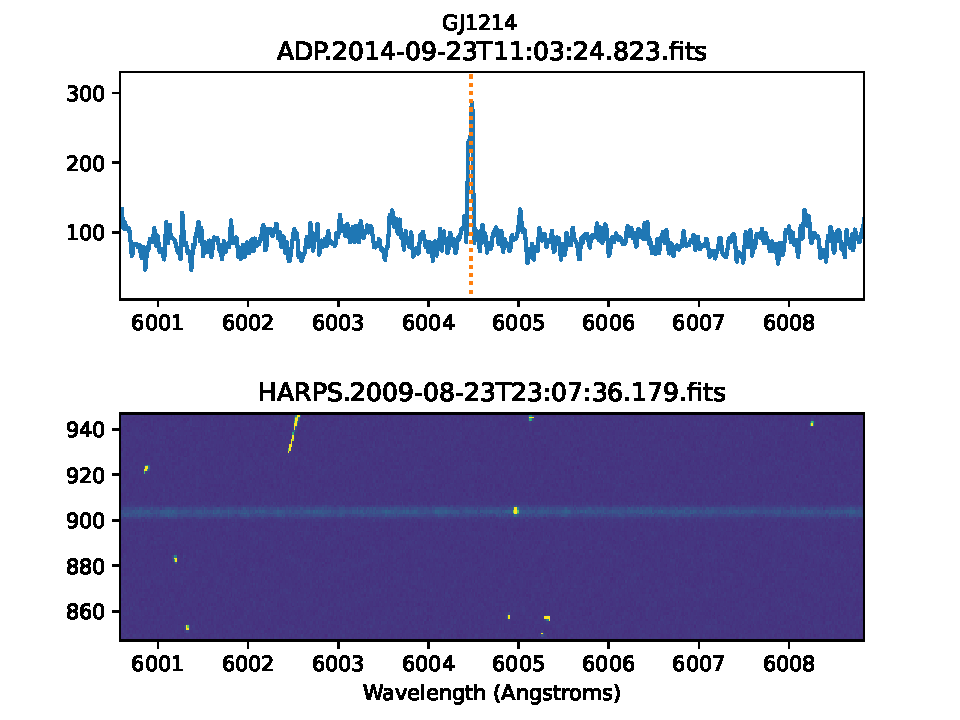
\includegraphics[width=.8\textwidth]{GJ1214_2009-08-23T23_07_36.179_6004.pdf}
    \caption{\DIFaddFL{Star: GJ-1214, Observation Date/Time: 2009-08-23 23:07:36.179. Top panel: reduced spectrum. Bottom panel: subsection of the corresponding CCD image for this wavelength range.}}
    \label{fig:figure_set}
\end{figure*}
\figsetstart
\figsetnum{17}
\figsettitle{{All Tier 4 Candidates}}
\figsetgrpstart
\figsetgrpnum{17.1}
\figsetgrptitle{BD-114672_2023-06-03T09_09_16.351_6477}
\figsetplot{BD-114672_2023-06-03T09_09_16.351_6477.pdf}
\figsetgrpnote{Star: BD-114672, Observation Date/Time: 2023-06-03 09:09:16. Top panel: reduced spectrum. Bottom panel: subsection of the corresponding CCD image for this wavelength range.}
\figsetgrpend
\figsetgrpstart
\figsetgrpnum{17.2}
\figsetgrptitle{CD-4911401_2005-05-10T04_34_42.474_6093}
\figsetplot{CD-4911401_2005-05-10T04_34_42.474_6093.pdf}
\figsetgrpnote{Star: CD-4911401, Observation Date/Time: 2005-05-10 04:34:42. Top panel: reduced spectrum. Bottom panel: subsection of the corresponding CCD image for this wavelength range.}
\figsetgrpend
\figsetgrpstart
\figsetgrpnum{17.3}
\figsetgrptitle{CoRoT-24_2009-11-28T06_10_56.607_6786}
\figsetplot{CoRoT-24_2009-11-28T06_10_56.607_6786.pdf}
\figsetgrpnote{Star: CoRoT-24, Observation Date/Time: 2009-11-28 06:10:56. Top panel: reduced spectrum. Bottom panel: subsection of the corresponding CCD image for this wavelength range.}
\figsetgrpend
\figsetgrpstart
\figsetgrpnum{17.4}
\figsetgrptitle{CoRoT-24_2010-02-12T01_24_19.113_5723}
\figsetplot{CoRoT-24_2010-02-12T01_24_19.113_5723.pdf}
\figsetgrpnote{Star: CoRoT-24, Observation Date/Time: 2010-02-12 01:24:19. Top panel: reduced spectrum. Bottom panel: subsection of the corresponding CCD image for this wavelength range.}
\figsetgrpend
\figsetgrpstart
\figsetgrpnum{17.5}
\figsetgrptitle{CoRoT-24_2010-02-17T03_34_56.067_6160}
\figsetplot{CoRoT-24_2010-02-17T03_34_56.067_6160.pdf}
\figsetgrpnote{Star: CoRoT-24, Observation Date/Time: 2010-02-17 03:34:56. Top panel: reduced spectrum. Bottom panel: subsection of the corresponding CCD image for this wavelength range.}
\figsetgrpend
\figsetgrpstart
\figsetgrpnum{17.6}
\figsetgrptitle{CoRoT-24_2011-11-08T07_17_18.816_6799}
\figsetplot{CoRoT-24_2011-11-08T07_17_18.816_6799.pdf}
\figsetgrpnote{Star: CoRoT-24, Observation Date/Time: 2011-11-08 07:17:18. Top panel: reduced spectrum. Bottom panel: subsection of the corresponding CCD image for this wavelength range.}
\figsetgrpend
\figsetgrpstart
\figsetgrpnum{17.7}
\figsetgrptitle{CoRoT-24_2011-11-23T05_50_42.823_4712}
\figsetplot{CoRoT-24_2011-11-23T05_50_42.823_4712.pdf}
\figsetgrpnote{Star: CoRoT-24, Observation Date/Time: 2011-11-23 05:50:42. Top panel: reduced spectrum. Bottom panel: subsection of the corresponding CCD image for this wavelength range.}
\figsetgrpend
\figsetgrpstart
\figsetgrpnum{17.8}
\figsetgrptitle{CoRoT-24_2011-11-23T05_50_42.823_5779}
\figsetplot{CoRoT-24_2011-11-23T05_50_42.823_5779.pdf}
\figsetgrpnote{Star: CoRoT-24, Observation Date/Time: 2011-11-23 05:50:42. Top panel: reduced spectrum. Bottom panel: subsection of the corresponding CCD image for this wavelength range.}
\figsetgrpend
\figsetgrpstart
\figsetgrpnum{17.9}
\figsetgrptitle{CoRoT-24_2011-11-24T04_34_33.827_6781}
\figsetplot{CoRoT-24_2011-11-24T04_34_33.827_6781.pdf}
\figsetgrpnote{Star: CoRoT-24, Observation Date/Time: 2011-11-24 04:34:33. Top panel: reduced spectrum. Bottom panel: subsection of the corresponding CCD image for this wavelength range.}
\figsetgrpend
\figsetgrpstart
\figsetgrpnum{17.10}
\figsetgrptitle{CoRoT-24_2011-11-26T05_55_33.755_6676}
\figsetplot{CoRoT-24_2011-11-26T05_55_33.755_6676.pdf}
\figsetgrpnote{Star: CoRoT-24, Observation Date/Time: 2011-11-26 05:55:33. Top panel: reduced spectrum. Bottom panel: subsection of the corresponding CCD image for this wavelength range.}
\figsetgrpend
\figsetgrpstart
\figsetgrpnum{17.11}
\figsetgrptitle{CoRoT-24_2011-12-04T05_29_17.513_5552}
\figsetplot{CoRoT-24_2011-12-04T05_29_17.513_5552.pdf}
\figsetgrpnote{Star: CoRoT-24, Observation Date/Time: 2011-12-04 05:29:17. Top panel: reduced spectrum. Bottom panel: subsection of the corresponding CCD image for this wavelength range.}
\figsetgrpend
\figsetgrpstart
\figsetgrpnum{17.12}
\figsetgrptitle{CoRoT-24_2011-12-04T05_29_17.513_5948}
\figsetplot{CoRoT-24_2011-12-04T05_29_17.513_5948.pdf}
\figsetgrpnote{Star: CoRoT-24, Observation Date/Time: 2011-12-04 05:29:17. Top panel: reduced spectrum. Bottom panel: subsection of the corresponding CCD image for this wavelength range.}
\figsetgrpend
\figsetgrpstart
\figsetgrpnum{17.13}
\figsetgrptitle{CoRoT-24_2011-12-05T04_42_05.773_6039}
\figsetplot{CoRoT-24_2011-12-05T04_42_05.773_6039.pdf}
\figsetgrpnote{Star: CoRoT-24, Observation Date/Time: 2011-12-05 04:42:05. Top panel: reduced spectrum. Bottom panel: subsection of the corresponding CCD image for this wavelength range.}
\figsetgrpend
\figsetgrpstart
\figsetgrpnum{17.14}
\figsetgrptitle{CoRoT-24_2012-01-14T04_55_44.391_5861}
\figsetplot{CoRoT-24_2012-01-14T04_55_44.391_5861.pdf}
\figsetgrpnote{Star: CoRoT-24, Observation Date/Time: 2012-01-14 04:55:44. Top panel: reduced spectrum. Bottom panel: subsection of the corresponding CCD image for this wavelength range.}
\figsetgrpend
\figsetgrpstart
\figsetgrpnum{17.15}
\figsetgrptitle{CoRoT-24_2012-01-16T01_46_11.545_5553}
\figsetplot{CoRoT-24_2012-01-16T01_46_11.545_5553.pdf}
\figsetgrpnote{Star: CoRoT-24, Observation Date/Time: 2012-01-16 01:46:11. Top panel: reduced spectrum. Bottom panel: subsection of the corresponding CCD image for this wavelength range.}
\figsetgrpend
\figsetgrpstart
\figsetgrpnum{17.16}
\figsetgrptitle{CoRoT-24_2012-01-18T04_23_59.478_5819}
\figsetplot{CoRoT-24_2012-01-18T04_23_59.478_5819.pdf}
\figsetgrpnote{Star: CoRoT-24, Observation Date/Time: 2012-01-18 04:23:59. Top panel: reduced spectrum. Bottom panel: subsection of the corresponding CCD image for this wavelength range.}
\figsetgrpend
\figsetgrpstart
\figsetgrpnum{17.17}
\figsetgrptitle{CoRoT-24_2012-01-19T01_47_54.198_6822}
\figsetplot{CoRoT-24_2012-01-19T01_47_54.198_6822.pdf}
\figsetgrpnote{Star: CoRoT-24, Observation Date/Time: 2012-01-19 01:47:54. Top panel: reduced spectrum. Bottom panel: subsection of the corresponding CCD image for this wavelength range.}
\figsetgrpend
\figsetgrpstart
\figsetgrpnum{17.18}
\figsetgrptitle{CoRoT-24_2012-01-22T04_12_46.138_6252}
\figsetplot{CoRoT-24_2012-01-22T04_12_46.138_6252.pdf}
\figsetgrpnote{Star: CoRoT-24, Observation Date/Time: 2012-01-22 04:12:46. Top panel: reduced spectrum. Bottom panel: subsection of the corresponding CCD image for this wavelength range.}
\figsetgrpend
\figsetgrpstart
\figsetgrpnum{17.19}
\figsetgrptitle{CoRoT-24_2012-01-25T01_49_25.109_6488}
\figsetplot{CoRoT-24_2012-01-25T01_49_25.109_6488.pdf}
\figsetgrpnote{Star: CoRoT-24, Observation Date/Time: 2012-01-25 01:49:25. Top panel: reduced spectrum. Bottom panel: subsection of the corresponding CCD image for this wavelength range.}
\figsetgrpend
\figsetgrpstart
\figsetgrpnum{17.20}
\figsetgrptitle{CoRoT-24_2012-11-17T04_56_35.576_5045}
\figsetplot{CoRoT-24_2012-11-17T04_56_35.576_5045.pdf}
\figsetgrpnote{Star: CoRoT-24, Observation Date/Time: 2012-11-17 04:56:35. Top panel: reduced spectrum. Bottom panel: subsection of the corresponding CCD image for this wavelength range.}
\figsetgrpend
\figsetgrpstart
\figsetgrpnum{17.21}
\figsetgrptitle{CoRoT-24_2012-11-20T05_56_02.541_5983}
\figsetplot{CoRoT-24_2012-11-20T05_56_02.541_5983.pdf}
\figsetgrpnote{Star: CoRoT-24, Observation Date/Time: 2012-11-20 05:56:02. Top panel: reduced spectrum. Bottom panel: subsection of the corresponding CCD image for this wavelength range.}
\figsetgrpend
\figsetgrpstart
\figsetgrpnum{17.22}
\figsetgrptitle{CoRoT-24_2012-11-24T06_04_07.004_5447}
\figsetplot{CoRoT-24_2012-11-24T06_04_07.004_5447.pdf}
\figsetgrpnote{Star: CoRoT-24, Observation Date/Time: 2012-11-24 06:04:07. Top panel: reduced spectrum. Bottom panel: subsection of the corresponding CCD image for this wavelength range.}
\figsetgrpend
\figsetgrpstart
\figsetgrpnum{17.23}
\figsetgrptitle{CoRoT-24_2012-11-24T06_04_07.004_5832}
\figsetplot{CoRoT-24_2012-11-24T06_04_07.004_5832.pdf}
\figsetgrpnote{Star: CoRoT-24, Observation Date/Time: 2012-11-24 06:04:07. Top panel: reduced spectrum. Bottom panel: subsection of the corresponding CCD image for this wavelength range.}
\figsetgrpend
\figsetgrpstart
\figsetgrpnum{17.24}
\figsetgrptitle{CoRoT-32_2012-01-27T02_14_50.135_6173}
\figsetplot{CoRoT-32_2012-01-27T02_14_50.135_6173.pdf}
\figsetgrpnote{Star: CoRoT-32, Observation Date/Time: 2012-01-27 02:14:50. Top panel: reduced spectrum. Bottom panel: subsection of the corresponding CCD image for this wavelength range.}
\figsetgrpend
\figsetgrpstart
\figsetgrpnum{17.25}
\figsetgrptitle{CoRoT101614469_2008-07-25T04_50_31.896_4534}
\figsetplot{CoRoT101614469_2008-07-25T04_50_31.896_4534.pdf}
\figsetgrpnote{Star: CoRoT101614469, Observation Date/Time: 2008-07-25 04:50:31. Top panel: reduced spectrum. Bottom panel: subsection of the corresponding CCD image for this wavelength range.}
\figsetgrpend
\figsetgrpstart
\figsetgrpnum{17.26}
\figsetgrptitle{CoRoT101614469_2008-07-25T04_50_31.896_5593}
\figsetplot{CoRoT101614469_2008-07-25T04_50_31.896_5593.pdf}
\figsetgrpnote{Star: CoRoT101614469, Observation Date/Time: 2008-07-25 04:50:31. Top panel: reduced spectrum. Bottom panel: subsection of the corresponding CCD image for this wavelength range.}
\figsetgrpend
\figsetgrpstart
\figsetgrpnum{17.27}
\figsetgrptitle{CoRoT101614469_2008-07-30T02_36_24.607_6689}
\figsetplot{CoRoT101614469_2008-07-30T02_36_24.607_6689.pdf}
\figsetgrpnote{Star: CoRoT101614469, Observation Date/Time: 2008-07-30 02:36:24. Top panel: reduced spectrum. Bottom panel: subsection of the corresponding CCD image for this wavelength range.}
\figsetgrpend
\figsetgrpstart
\figsetgrpnum{17.28}
\figsetgrptitle{CoRoT221699621_2011-02-24T00_46_36.187_6416}
\figsetplot{CoRoT221699621_2011-02-24T00_46_36.187_6416.pdf}
\figsetgrpnote{Star: CoRoT221699621, Observation Date/Time: 2011-02-24 00:46:36. Top panel: reduced spectrum. Bottom panel: subsection of the corresponding CCD image for this wavelength range.}
\figsetgrpend
\figsetgrpstart
\figsetgrpnum{17.29}
\figsetgrptitle{CoRoT221699621_2011-12-02T06_21_36.140_6716}
\figsetplot{CoRoT221699621_2011-12-02T06_21_36.140_6716.pdf}
\figsetgrpnote{Star: CoRoT221699621, Observation Date/Time: 2011-12-02 06:21:36. Top panel: reduced spectrum. Bottom panel: subsection of the corresponding CCD image for this wavelength range.}
\figsetgrpend
\figsetgrpstart
\figsetgrpnum{17.30}
\figsetgrptitle{CoRoT221699621_2011-12-03T06_43_16.408_5446}
\figsetplot{CoRoT221699621_2011-12-03T06_43_16.408_5446.pdf}
\figsetgrpnote{Star: CoRoT221699621, Observation Date/Time: 2011-12-03 06:43:16. Top panel: reduced spectrum. Bottom panel: subsection of the corresponding CCD image for this wavelength range.}
\figsetgrpend
\figsetgrpstart
\figsetgrpnum{17.31}
\figsetgrptitle{GJ1214_2009-07-26T00_32_36.836_6113}
\figsetplot{GJ1214_2009-07-26T00_32_36.836_6113.pdf}
\figsetgrpnote{Star: GJ1214, Observation Date/Time: 2009-07-26 00:32:36. Top panel: reduced spectrum. Bottom panel: subsection of the corresponding CCD image for this wavelength range.}
\figsetgrpend
\figsetgrpstart
\figsetgrpnum{17.32}
\figsetgrptitle{GJ1214_2009-08-05T00_48_08.218_3972}
\figsetplot{GJ1214_2009-08-05T00_48_08.218_3972.pdf}
\figsetgrpnote{Star: GJ1214, Observation Date/Time: 2009-08-05 00:48:08. Top panel: reduced spectrum. Bottom panel: subsection of the corresponding CCD image for this wavelength range.}
\figsetgrpend
\figsetgrpstart
\figsetgrpnum{17.33}
\figsetgrptitle{GJ1214_2009-08-23T23_07_36.179_6004}
\figsetplot{GJ1214_2009-08-23T23_07_36.179_6004.pdf}
\figsetgrpnote{Star: GJ1214, Observation Date/Time: 2009-08-23 23:07:36. Top panel: reduced spectrum. Bottom panel: subsection of the corresponding CCD image for this wavelength range.}
\figsetgrpend
\figsetgrpstart
\figsetgrpnum{17.34}
\figsetgrptitle{GJ1214_2009-09-03T23_26_05.655_4527}
\figsetplot{GJ1214_2009-09-03T23_26_05.655_4527.pdf}
\figsetgrpnote{Star: GJ1214, Observation Date/Time: 2009-09-03 23:26:05. Top panel: reduced spectrum. Bottom panel: subsection of the corresponding CCD image for this wavelength range.}
\figsetgrpend
\figsetgrpstart
\figsetgrpnum{17.35}
\figsetgrptitle{GJ1214_2012-07-10T00_39_39.961_4784}
\figsetplot{GJ1214_2012-07-10T00_39_39.961_4784.pdf}
\figsetgrpnote{Star: GJ1214, Observation Date/Time: 2012-07-10 00:39:39. Top panel: reduced spectrum. Bottom panel: subsection of the corresponding CCD image for this wavelength range.}
\figsetgrpend
\figsetgrpstart
\figsetgrpnum{17.36}
\figsetgrptitle{GJ1214_2012-07-13T00_55_14.696_3897}
\figsetplot{GJ1214_2012-07-13T00_55_14.696_3897.pdf}
\figsetgrpnote{Star: GJ1214, Observation Date/Time: 2012-07-13 00:55:14. Top panel: reduced spectrum. Bottom panel: subsection of the corresponding CCD image for this wavelength range.}
\figsetgrpend
\figsetgrpstart
\figsetgrpnum{17.37}
\figsetgrptitle{GJ1214_2012-09-02T00_18_54.276_4076}
\figsetplot{GJ1214_2012-09-02T00_18_54.276_4076.pdf}
\figsetgrpnote{Star: GJ1214, Observation Date/Time: 2012-09-02 00:18:54. Top panel: reduced spectrum. Bottom panel: subsection of the corresponding CCD image for this wavelength range.}
\figsetgrpend
\figsetgrpstart
\figsetgrpnum{17.38}
\figsetgrptitle{GJ1214_2012-09-21T23_44_14.907_5804}
\figsetplot{GJ1214_2012-09-21T23_44_14.907_5804.pdf}
\figsetgrpnote{Star: GJ1214, Observation Date/Time: 2012-09-21 23:44:14. Top panel: reduced spectrum. Bottom panel: subsection of the corresponding CCD image for this wavelength range.}
\figsetgrpend
\figsetgrpstart
\figsetgrpnum{17.39}
\figsetgrptitle{GJ1214_2019-07-15T03_32_39.231_4629}
\figsetplot{GJ1214_2019-07-15T03_32_39.231_4629.pdf}
\figsetgrpnote{Star: GJ1214, Observation Date/Time: 2019-07-15 03:32:39. Top panel: reduced spectrum. Bottom panel: subsection of the corresponding CCD image for this wavelength range.}
\figsetgrpend
\figsetgrpstart
\figsetgrpnum{17.40}
\figsetgrptitle{GJ1214_2019-09-02T01_26_36.055_5432}
\figsetplot{GJ1214_2019-09-02T01_26_36.055_5432.pdf}
\figsetgrpnote{Star: GJ1214, Observation Date/Time: 2019-09-02 01:26:36. Top panel: reduced spectrum. Bottom panel: subsection of the corresponding CCD image for this wavelength range.}
\figsetgrpend
\figsetgrpstart
\figsetgrpnum{17.41}
\figsetgrptitle{GJ1236_2012-05-15T07_27_46.968_5975}
\figsetplot{GJ1236_2012-05-15T07_27_46.968_5975.pdf}
\figsetgrpnote{Star: GJ1236, Observation Date/Time: 2012-05-15 07:27:46. Top panel: reduced spectrum. Bottom panel: subsection of the corresponding CCD image for this wavelength range.}
\figsetgrpend
\figsetgrpstart
\figsetgrpnum{17.42}
\figsetgrptitle{GJ3053_2016-01-23T01_11_31.273_3854}
\figsetplot{GJ3053_2016-01-23T01_11_31.273_3854.pdf}
\figsetgrpnote{Star: GJ3053, Observation Date/Time: 2016-01-23 01:11:31. Top panel: reduced spectrum. Bottom panel: subsection of the corresponding CCD image for this wavelength range.}
\figsetgrpend
\figsetgrpstart
\figsetgrpnum{17.43}
\figsetgrptitle{GJ317_2018-04-10T03_25_08.275_4662}
\figsetplot{GJ317_2018-04-10T03_25_08.275_4662.pdf}
\figsetgrpnote{Star: GJ317, Observation Date/Time: 2018-04-10 03:25:08. Top panel: reduced spectrum. Bottom panel: subsection of the corresponding CCD image for this wavelength range.}
\figsetgrpend
\figsetgrpstart
\figsetgrpnum{17.44}
\figsetgrptitle{GJ317_2018-06-01T22_30_16.020_6643}
\figsetplot{GJ317_2018-06-01T22_30_16.020_6643.pdf}
\figsetgrpnote{Star: GJ317, Observation Date/Time: 2018-06-01 22:30:16. Top panel: reduced spectrum. Bottom panel: subsection of the corresponding CCD image for this wavelength range.}
\figsetgrpend
\figsetgrpstart
\figsetgrpnum{17.45}
\figsetgrptitle{GJ3221_2011-09-25T07_25_30.812_6688}
\figsetplot{GJ3221_2011-09-25T07_25_30.812_6688.pdf}
\figsetgrpnote{Star: GJ3221, Observation Date/Time: 2011-09-25 07:25:30. Top panel: reduced spectrum. Bottom panel: subsection of the corresponding CCD image for this wavelength range.}
\figsetgrpend
\figsetgrpstart
\figsetgrpnum{17.46}
\figsetgrptitle{GJ3535_2004-05-31T00_36_26.077_6769}
\figsetplot{GJ3535_2004-05-31T00_36_26.077_6769.pdf}
\figsetgrpnote{Star: GJ3535, Observation Date/Time: 2004-05-31 00:36:26. Top panel: reduced spectrum. Bottom panel: subsection of the corresponding CCD image for this wavelength range.}
\figsetgrpend
\figsetgrpstart
\figsetgrpnum{17.47}
\figsetgrptitle{HD110411_2006-02-10T07_02_59.081_5709}
\figsetplot{HD110411_2006-02-10T07_02_59.081_5709.pdf}
\figsetgrpnote{Star: HD110411, Observation Date/Time: 2006-02-10 07:02:59. Top panel: reduced spectrum. Bottom panel: subsection of the corresponding CCD image for this wavelength range.}
\figsetgrpend
\figsetgrpstart
\figsetgrpnum{17.48}
\figsetgrptitle{HD147644_2015-04-19T06_48_21.114_5937}
\figsetplot{HD147644_2015-04-19T06_48_21.114_5937.pdf}
\figsetgrpnote{Star: HD147644, Observation Date/Time: 2015-04-19 06:48:21. Top panel: reduced spectrum. Bottom panel: subsection of the corresponding CCD image for this wavelength range.}
\figsetgrpend
\figsetgrpstart
\figsetgrpnum{17.49}
\figsetgrptitle{HD184711_2008-09-20T00_41_44.834_6566}
\figsetplot{HD184711_2008-09-20T00_41_44.834_6566.pdf}
\figsetgrpnote{Star: HD184711, Observation Date/Time: 2008-09-20 00:41:44. Top panel: reduced spectrum. Bottom panel: subsection of the corresponding CCD image for this wavelength range.}
\figsetgrpend
\figsetgrpstart
\figsetgrpnum{17.50}
\figsetgrptitle{HD197623_2005-05-18T09_10_45.139_6351}
\figsetplot{HD197623_2005-05-18T09_10_45.139_6351.pdf}
\figsetgrpnote{Star: HD197623, Observation Date/Time: 2005-05-18 09:10:45. Top panel: reduced spectrum. Bottom panel: subsection of the corresponding CCD image for this wavelength range.}
\figsetgrpend
\figsetgrpstart
\figsetgrpnum{17.51}
\figsetgrptitle{HD223171_2015-12-16T01_26_43.087_6769}
\figsetplot{HD223171_2015-12-16T01_26_43.087_6769.pdf}
\figsetgrpnote{Star: HD223171, Observation Date/Time: 2015-12-16 01:26:43. Top panel: reduced spectrum. Bottom panel: subsection of the corresponding CCD image for this wavelength range.}
\figsetgrpend
\figsetgrpstart
\figsetgrpnum{17.52}
\figsetgrptitle{HD34642_2018-02-01T01_42_30.839_5769}
\figsetplot{HD34642_2018-02-01T01_42_30.839_5769.pdf}
\figsetgrpnote{Star: HD34642, Observation Date/Time: 2018-02-01 01:42:30. Top panel: reduced spectrum. Bottom panel: subsection of the corresponding CCD image for this wavelength range.}
\figsetgrpend
\figsetgrpstart
\figsetgrpnum{17.53}
\figsetgrptitle{HD59088_2006-03-26T00_02_33.378_4365}
\figsetplot{HD59088_2006-03-26T00_02_33.378_4365.pdf}
\figsetgrpnote{Star: HD59088, Observation Date/Time: 2006-03-26 00:02:33. Top panel: reduced spectrum. Bottom panel: subsection of the corresponding CCD image for this wavelength range.}
\figsetgrpend
\figsetgrpstart
\figsetgrpnum{17.54}
\figsetgrptitle{HIP60910_2019-02-17T08_19_27.734_4305}
\figsetplot{HIP60910_2019-02-17T08_19_27.734_4305.pdf}
\figsetgrpnote{Star: HIP60910, Observation Date/Time: 2019-02-17 08:19:27. Top panel: reduced spectrum. Bottom panel: subsection of the corresponding CCD image for this wavelength range.}
\figsetgrpend
\figsetgrpstart
\figsetgrpnum{17.55}
\figsetgrptitle{HIP87607_2012-10-22T23_39_09.238_4632}
\figsetplot{HIP87607_2012-10-22T23_39_09.238_4632.pdf}
\figsetgrpnote{Star: HIP87607, Observation Date/Time: 2012-10-22 23:39:09. Top panel: reduced spectrum. Bottom panel: subsection of the corresponding CCD image for this wavelength range.}
\figsetgrpend
\figsetgrpstart
\figsetgrpnum{17.56}
\figsetgrptitle{HIP87607_2013-07-24T02_37_41.553_5674}
\figsetplot{HIP87607_2013-07-24T02_37_41.553_5674.pdf}
\figsetgrpnote{Star: HIP87607, Observation Date/Time: 2013-07-24 02:37:41. Top panel: reduced spectrum. Bottom panel: subsection of the corresponding CCD image for this wavelength range.}
\figsetgrpend
\figsetgrpstart
\figsetgrpnum{17.57}
\figsetgrptitle{WASP-19_2010-03-19T04_02_37.912_5948}
\figsetplot{WASP-19_2010-03-19T04_02_37.912_5948.pdf}
\figsetgrpnote{Star: WASP-19, Observation Date/Time: 2010-03-19 04:02:37. Top panel: reduced spectrum. Bottom panel: subsection of the corresponding CCD image for this wavelength range.}
\figsetgrpend
\figsetgrpstart
\figsetgrpnum{17.58}
\figsetgrptitle{WASP-19_2010-03-19T05_41_10.913_6859}
\figsetplot{WASP-19_2010-03-19T05_41_10.913_6859.pdf}
\figsetgrpnote{Star: WASP-19, Observation Date/Time: 2010-03-19 05:41:10. Top panel: reduced spectrum. Bottom panel: subsection of the corresponding CCD image for this wavelength range.}
\figsetgrpend
\figsetgrpstart
\figsetgrpnum{17.59}
\figsetgrptitle{WASP-19_2017-05-09T00_23_21.566_5988}
\figsetplot{WASP-19_2017-05-09T00_23_21.566_5988.pdf}
\figsetgrpnote{Star: WASP-19, Observation Date/Time: 2017-05-09 00:23:21. Top panel: reduced spectrum. Bottom panel: subsection of the corresponding CCD image for this wavelength range.}
\figsetgrpend
\figsetgrpstart
\figsetgrpnum{17.60}
\figsetgrptitle{WASP-19_2020-02-14T03_38_48.531_4245}
\figsetplot{WASP-19_2020-02-14T03_38_48.531_4245.pdf}
\figsetgrpnote{Star: WASP-19, Observation Date/Time: 2020-02-14 03:38:48. Top panel: reduced spectrum. Bottom panel: subsection of the corresponding CCD image for this wavelength range.}
\figsetgrpend
\figsetgrpstart
\figsetgrpnum{17.61}
\figsetgrptitle{WASP-19_2020-02-15T04_09_40.886_6054}
\figsetplot{WASP-19_2020-02-15T04_09_40.886_6054.pdf}
\figsetgrpnote{Star: WASP-19, Observation Date/Time: 2020-02-15 04:09:40. Top panel: reduced spectrum. Bottom panel: subsection of the corresponding CCD image for this wavelength range.}
\figsetgrpend
\figsetgrpstart
\figsetgrpnum{17.62}
\figsetgrptitle{WASP-89_2012-10-03T03_54_35.331_4925}
\figsetplot{WASP-89_2012-10-03T03_54_35.331_4925.pdf}
\figsetgrpnote{Star: WASP-89, Observation Date/Time: 2012-10-03 03:54:35. Top panel: reduced spectrum. Bottom panel: subsection of the corresponding CCD image for this wavelength range.}
\figsetgrpend
\figsetgrpstart
\figsetgrpnum{17.63}
\figsetgrptitle{WASP-89_2012-10-03T05_01_01.142_5198}
\figsetplot{WASP-89_2012-10-03T05_01_01.142_5198.pdf}
\figsetgrpnote{Star: WASP-89, Observation Date/Time: 2012-10-03 05:01:01. Top panel: reduced spectrum. Bottom panel: subsection of the corresponding CCD image for this wavelength range.}
\figsetgrpend
\figsetgrpstart
\figsetgrpnum{17.64}
\figsetgrptitle{WASP-89_2013-06-15T05_34_26.988_5939}
\figsetplot{WASP-89_2013-06-15T05_34_26.988_5939.pdf}
\figsetgrpnote{Star: WASP-89, Observation Date/Time: 2013-06-15 05:34:26. Top panel: reduced spectrum. Bottom panel: subsection of the corresponding CCD image for this wavelength range.}
\figsetgrpend
\figsetgrpstart
\figsetgrpnum{17.65}
\figsetgrptitle{WASP-89_2013-06-15T05_49_59.413_6560}
\figsetplot{WASP-89_2013-06-15T05_49_59.413_6560.pdf}
\figsetgrpnote{Star: WASP-89, Observation Date/Time: 2013-06-15 05:49:59. Top panel: reduced spectrum. Bottom panel: subsection of the corresponding CCD image for this wavelength range.}
\figsetgrpend
\figsetgrpstart
\figsetgrpnum{17.66}
\figsetgrptitle{WASP-89_2013-06-15T07_38_42.423_6297}
\figsetplot{WASP-89_2013-06-15T07_38_42.423_6297.pdf}
\figsetgrpnote{Star: WASP-89, Observation Date/Time: 2013-06-15 07:38:42. Top panel: reduced spectrum. Bottom panel: subsection of the corresponding CCD image for this wavelength range.}
\figsetgrpend
\figsetgrpstart
\figsetgrpnum{17.67}
\figsetgrptitle{WASP-89_2013-06-15T08_09_45.993_6551}
\figsetplot{WASP-89_2013-06-15T08_09_45.993_6551.pdf}
\figsetgrpnote{Star: WASP-89, Observation Date/Time: 2013-06-15 08:09:45. Top panel: reduced spectrum. Bottom panel: subsection of the corresponding CCD image for this wavelength range.}
\figsetgrpend
\figsetend
\DIFaddend 

\bibliographystyle{aasjournalv7}
\bibliography{references.bib}

\end{document}
